% ----------------------------------------------
% \section{Introduction}
\label{sec:intro}

Here we will consider the effect of noise correlations in V1 and V4 on the information contained within the firing rates across a population of 20--30 neurons and how this changes with perceptual learning.
First we will consider how noise correlations between pairs of neurons changes with learning. Then we will apply a decoder to the spike rate data and investigate how the performance of the decoder changes with learning. We will also investigate how the noise correlations impact the decoder and whether this changes with learning.

% ----------------------------------------------
\section{Background}

The firing rate of neurons in the sensory system will vary trial-to-trial, even if the stimulus presented is the same. The manner in which these responses fluctuate together is known as the noise correlation between neurons. If there are positive noise correlations, the changes in neural activity across a population will increase and decrease together. Long-standing theoretical work has indicated such correlations will hamper the ability of upstream neurons to accurately decode the stimulus% [cite]
, which is in keeping with experimental results demonstrating attention reduces noise correlations \citep{Cohen2009}. This fits with intuition --- if stimulus A is encoded with one firing rate across a population and stimulus B with a slightly higher rate, a systematic increase or decrease in the population firing rates can easily cause A and B to be confused with one another. However, recent theoretical results indicate that for a more realistic non-homogeneous population of neurons, neural correlations do not limit the population-wide information as the number of neurons increases \citep{Oram1998,Averbeck2006,Ecker2011}.
A recent paper by \citet{Gu2011} on neurons recoded from the macaque dorsal medial superior temporal area (MSTd) before and after training in a head direction discrimination task, found that although pairwise noise correlations between neurons are reduced with training, this does not yield an increase in performance in a decoder. We will see if these findings hold here as well.

% ----------------------------------------------
\section{Methods}
% ----------------------------------------------

% ----------------------------------------------
\subsection{Linear Decoder}
\label{sec:dec-meth-lin}

The input data to the decoding algorithm was chosen to be the total spike count during stimulus presentation from each trial. This total is taken only for channels known to offer a consistent firing rate across sessions after the spontaneous activity matching process. If there are 20 such channels in the dataset, taking the total number of spikes during stimulus presentation for each of the channels results in a 20-dimensional vector of population activity on each trial.

It should be noted that using all the spikes during the stimulus presentation period is likely to be sub-optimal, as not necessarily all of this period of time is carrying useful information about the stimuli. The amount of spikes before the onset response, for instance, is clearly not stimulus dependent as it precedes the neural response to the stimulus, so it will only be a source of noise and  not useful for the decoding.
Furthermore, it is possible that the firing rate during the onset response might be more informative than the average firing rate across the whole presentation period. However, finding the optimal window from which to take the spikes is an exercise in of itself.

The decoder used was a Fisher linear discriminant classifier. Given a training dataset of labelled datapoints in 20D, the classifier will find the optimal 19D hyperplane such that it separates the two classes of points optimally, under the assumption that the two clusters to be separated are multivariate normal distributions. The vector normal to the hyperplane is 
\begin{equation}
\vec{w} = \Sigma^{-1}\left(\vec{\mu_1}-\vec{\mu_0}\right)
\end{equation}
where $\Sigma$ is the covariance matrix between the two populations, as determined from the available labelled data, and $\vec{\mu_0}$ and $\vec{\mu_1}$ are the computed means of the two distributions.

Once a classifying hyperplane has been found, test datapoints can be classified by observing the side of the hyperplane on which they fall. For a new datapoint, $\vec{x}$,  if
\begin{equation}
\vec{w}\cdot\vec{x}>c
\end{equation}
then we classify $\vec{x}$ as group 1 (higher than 30\% contrast), otherwise we classify it as 0 (lower).

This was performed using the function \texttt{classify} with type `linear' in MATLAB. For training and testing of the decoder, leave-one-out classification was used across each session individually. This means that for a session of 500 trials, the decoder is trained on 499 trials with the spike counts for all the trials and the correct response (higher or lower than 30\% contrast) and we then check whether the decoder identifies the remaining trial correctly.
This is repeated for all the 500 trials, and then the performance is defined as the proportion of trials which are identified correctly. Training the decoder in this way means the decoding hyperplane used for classification is optimal for each individual session, but also different for each session.

The impact of noise correlations on the decoder is considered by comparing the regular decoder performance with the performance of a decoder applied to data which has been shuffled across trials under the same stimulus conditions. After shuffling, specific neural response vectors no longer correspond to any particular trial, since the spike counts for each channel are taken from different trials.

% ----------------------------------------------
\subsection{Probabilistic Model}
\label{sec:dec-meth-prob}

As well as comparing the behavioural and decoding responses with the target responses to find a value for predictor perforance, we can compare the behavioural and decoding responses with one another and find a value for their agreement, the proportion of trials on which the two responses are the same.

We would like to evaluate whether the behavioural respones are dependent on the firing rates of the recorded population of neurons. This can be done by considering the behavioural and decoding response agreement, but in order to do this we need to contstruct a model of how much agreement we would expect to find if the two were completely independent, which will form our null hypothesis (NH) to compare against.

Throughout this work, it is assumed that the behavioural and decoding responses are given by a Bernoulli distribution. In this model, there is a true probability, $p$, of the animal giving the correct answer to the task for each trial, which is sampled from on each of the trials. When this is sampled over $n$ trials, we expect to find $np$ trials have been responded correctly and $n(1-p)$ incorrectly.

Hence the underlying true probability of a correct response can be approximated by taking the number of correct responses and dividing them by the total number of trials. Using one of several statistical methods, we can find an estimate for a percentage confidence interval (PCI).
It is from this that error bars, indicated by the shaded regions surrounding line plots in Figs.~\ref{fig:dec_all_v1} and ~\ref{fig:dec_all_v4}, are computed. These are presented as the standard error, equivalent to a 31.8\%  confidence interval within which 68.2\% of datapoints are expected to lie. (This has been done using the function \texttt{binofit} in MATLAB, which utilises the Clopper-Pearson method. Although this is not the best method, it should be sufficient for our purposes.)

The behavioural performance is given by the estimated probability of the behavioural response being the same as the correct response, simply found by dividing the number of times the behavioural response matched the target response by the number of presentations.
The target response is of course whether or not the test stimulus is actually higher or lower than the sample. Similarly, the decoding performance is the proportion of times the decoding response is the same as the target response; and the behavioural and decoding agreement is the proportion of times the behavioural and decoding responses are the same.

Using the estimated probabilities of the behavioural and decoding responses being correct, we can find an expected agreement between the behavioural and decoding responses if they are completely independent of one another, which constitutes the null hypothesis model (NH). By comparing the observed agreement with the agreement we expect for independent variables, we can see whether or not behavioural responses are correlated with the decoded neural responses.

The theory behind the estimation of the agreement for independent binomial processes is described as follows. Let us take two independent binomial variables, $X_1$ and $X_2$, which can either be in state $s_1$ with probabilities $p_1$ and $p_2$ respectively, or in state $s_2$ with probability $(1-p_1)$ and $(1-p_2)$.
If $X_1$ and $X_2$ are completely independent, we expect to find them in the same state with probability $p_1 \, p_2 + (1-p_1) (1-p_2)$. Obviously, if $p_1$ and $p_2$ are both 0.5, there is a 0.5 chance of them being in the same state.
If $p_1$ and $p_2$ are both either higher or lower than 0.5, there is a higher chance of $X_1$ and $X_2$ being in the same state, and conversely if one is above and one below 0.5, there is a lower chance of them being in the same state. This means that if the probabilities of the behavioural and decoding responses being correct rises during the perceptual learning process, we expect the proportion of trials on which they agree to rise as well, even if the two distributions are completely independent.

The initial model for the expected agreement between behaviour and decoding used a simple model as described above, where $p_1$ and $p_2$ are taken to be the overall probability of a correct response across all the test stimuli for behaviour and decoding respectively. We will refer to this model as the single binomial model, as each predictor is modelled with a single binomial.
However, since there are 14 possible stimuli with varying difficulty, a more detailed model can be conceived in which the probability of a correct response for each predictor depends on the stimulus presented. In this ``multi-binomial'' model, the set of conditions (different stimuli) is given by $C$, and each predictor, $i\in\{b,d\}$, can either be in the ``lower'' or ``higher'' state ($s_l$ or $s_h$).
For each $c\in C$, there is some probability $p_{il|c} := P(x_i=s_l|c)$ of predictor a being in the lower state. Consequently, the probability of the two predictors being in the same state is given by
$$p_a = \sum_{c\in C} P(c) (p_{bl|c} \, p_{dl|c} + (1-p_{bl|c}) (1-p_{dl|c}),$$
where $P(c)$ is the probability of condition $c$ being presented to the animal on any given trial.

We will assume that $c$ is a random variable, which is sampled from for each trial independent from prior trials. This is a simplification of the actual condition selection process, ``delayed repetition''. In this, the conditions for a set of trials are chosen in advance with $n$ appearances of each condition in a random order, after which any trial on which the animal responded incorrectly is repeated. This means the single random variable approximation $P(c)$ is not uniform across the conditions, as harder conditions are presented more frequently.

For a given group of trials (such as, for instance, a single session), $P(c)$ can be estimated by dividing the number of times each appears by the total number of trials in the group. Similarly, $p_{il|c}$ can be estimated by dividing the number of trials on which the predictor was in the lower state for a given condition by the number of trials where that condition was presented.

It is not immediately clear whether the single- or multi-binomial models will yield similar or different results. Obviously, the multi-binomial model has more accurate detail and so should give a better result, but whether or not the single binomial should give a reasonable approximation is not obvious, though one would assume it would.
Applying the two models to the data and comparing them, we found the single binomial significantly underestimates the agreement which would really be found if the two predictors were completely independent. Henceforth, only the more accurate multi-binomial model is considered.

The expected agreement under the assumption of two independent binomial processes gives us the null hypothesis model to compare against. If the results of the analysis deviate significantly from this model, we can conclude the behavioural and neural decoded responses are correlated. A $p<0.05$ significance boundary was found by sampling the NH model 100,000 times and noting the agreement for the fifth-percentile of samples. During this sampling, the number of trials for each test condition was fixed with the same values as used in the experiment. Since we are only interested in sessions where the behavioural and decoded responses agree more than they would if independent, a single-tailed test was used. (NB: in the figures below, the single-tailed lower bound is also included for symmetry, so only 90\% of the samples lie within the shaded region).

The multi-binomial model should not be confused with a multinomial distribution, which would map one random variable to $n$ possible responses. The model used here is instead a two-step process where there are a set of binomial distributions, which binomial is used is determined by one random variable (the output of which is the same for both behaviour and decoder), and the output of the selected binomial is given by a second random variable. In essence, the simple, single binomial model is similar to shuffling the responses across all trials regardless of condition, and the multi-binomial model we use is similar to shuffling the responses with the same condition presented.

% ----------------------------------------------
\subsection{Noise correlations}
\label{sec:dec-meth-noise}

The noise correlation was investigated by considering how strongly correlated the spike counts during test stimulus presentation.
% (this could have been done using the data from the sample presentation, which would probably have been a better idea).

To evaluate the strength of noise correlations, the Pearson $r$ correlation coefficient was used. For two random variables $X$ and $Y$, this is given by
$$r_{X,Y} = \frac{\operatorname{cov}(X,Y)}{\sigma_X \, \sigma_Y}$$
and provides a version of the covariance between the $X$ and $Y$ which is normalised again their standard deviations.
This means $-1 \le r \le 1$ indicates how well $X$ and $Y$ fit a straight line relationship of either positive or negative slope, regardless of the gradient of the line, which could be changed by rescaling either $X$ or $Y$. If $r=\pm1$, there is a perfect linear relationship between $X$ and $Y$, whilst if $r=0$ then $X$ and $Y$ are completely independent.

For each individual session, the Pearson $r$ correlation coefficient was computed between the spike counts during test stimulus presentation between pairs of channels, across all the trials in the session. $r$ was computed for each pair and each condition, and the mean was taken across all of these.

As noted previously, on some trials movements of the subject produced a recording artifact across multiple channels which was incorrectly registered as genuine spikes by the spike detection algorithm. When comparing the spike counts for a pair of channels, to trials with erroneously high detected spike rates for both channels, as shown in Fig.~\ref{fig:noise_scatter}.

\begin{figure}[htbp]
\centering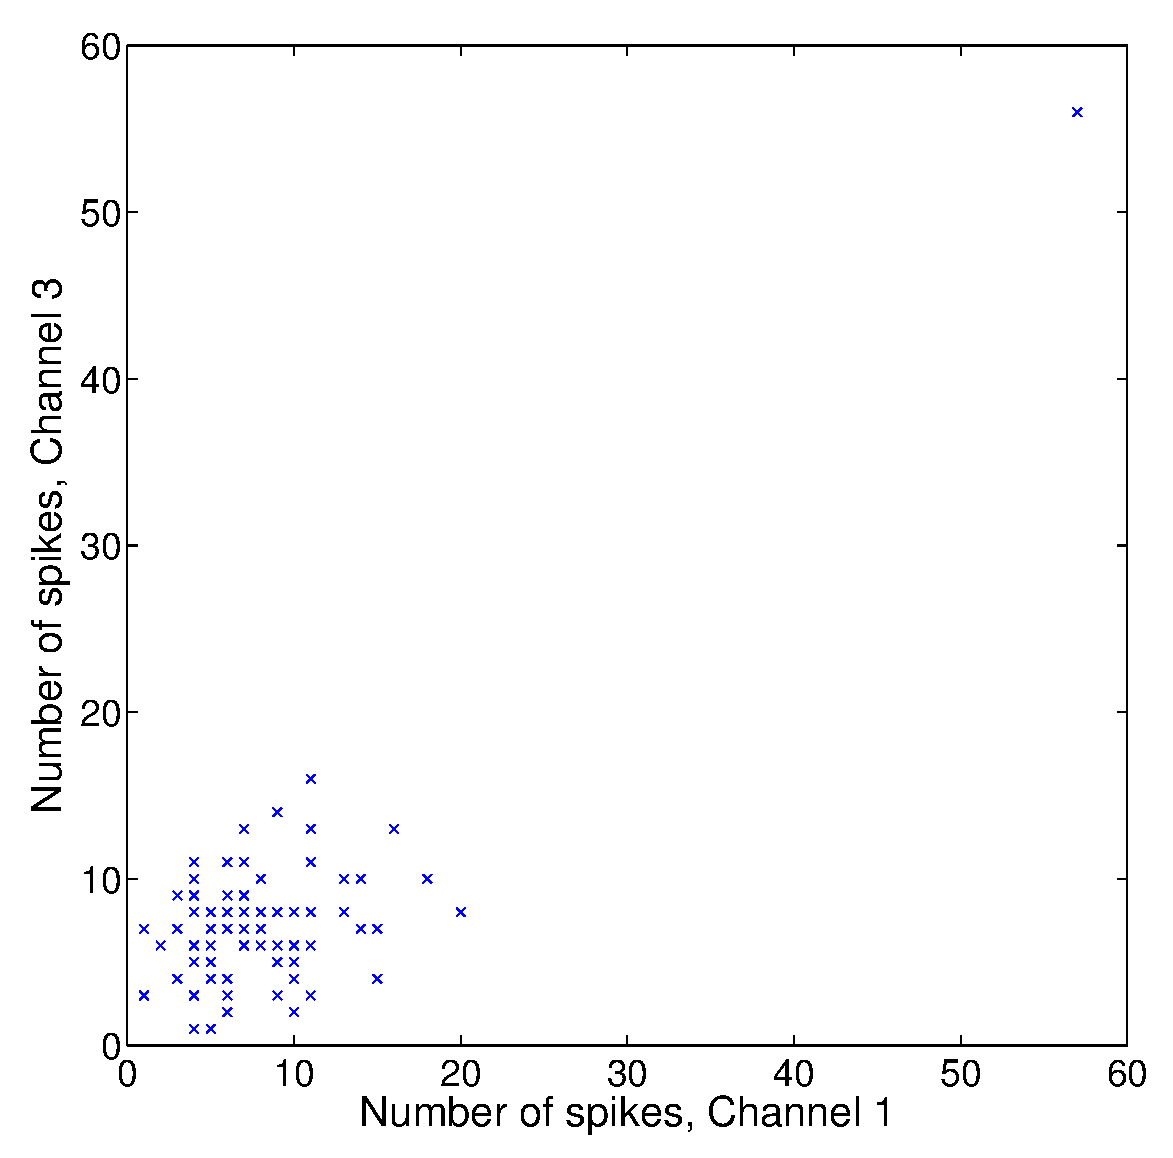
\includegraphics[width=0.4\linewidth]{%
./figs/decoding/rcoef_scatter_jv4_icond5_ch1vch3.eps}
\caption{Spikes count during around 500ms of presentation of the 27\% contrast stimulus, for two channels plotted against each other. There is clearly a weak correlation between the two data-series, but one trial is an outlier with a large number of measured spikes for both channels due to a correlated source of noise in the raw signal. The outlier will cause the correlation to be measured anomalously high.}
\label{fig:noise_scatter}
\end{figure}

To counter this problem, all trials where at least a quarter of the channels had a number of spikes more than 2.5 standard deviations above their mean spike count were removed. This should be effective at fixing the problem because the motion-triggered artifact occurs always effects multiple channels simultaneously with the same artifact.

% ----------------------------------------------
\section{Results}
% ----------------------------------------------

% ----------------------------------------------
% \clearpage
\subsection{Decoding}

Fig.~\ref{fig:dec_singles} shows how well the decoder does based only on data from individual channels. The performance was measured as described in \S\ref{sec:dec-meth-lin} for each session, and then averaged over all sessions. [perhaps a histogram would show how these are distributed better?]

Fig.~\ref{fig:dec_nbest} indicates how the performance of the decoder improves as more channels are added. We can see that the decoder performance saturates after around 10 channels are included in the training data, but at a perforance which is still far from the ideal. After this, including additional channels yields only a slight increase in performance, suggesting nearly all the information contained in the remaining channels is redundant, as it has already been given in the first 10 channels. [would be better to look at how the decoding perfarmance is distributed across all possible sets of $n$ channels, rather than just the best set of $n$ channels] [this should be compared with shuffled data to see what the impact is and whether performance does not saturate when correlations are removed as per some previous papers [cite]]

NB: the order in which channels were added in Fig.~\ref{fig:dec_nbest} is not the same ordering as they are shown in Fig.~\ref{fig:dec_singles}.

% % \begin{figure}[htbp]
% %     \begin{subfigure}[b]{0.5\linewidth}
% %         \centering
% %         \caption{}
% %         \label{fig:dec_singles}
% %         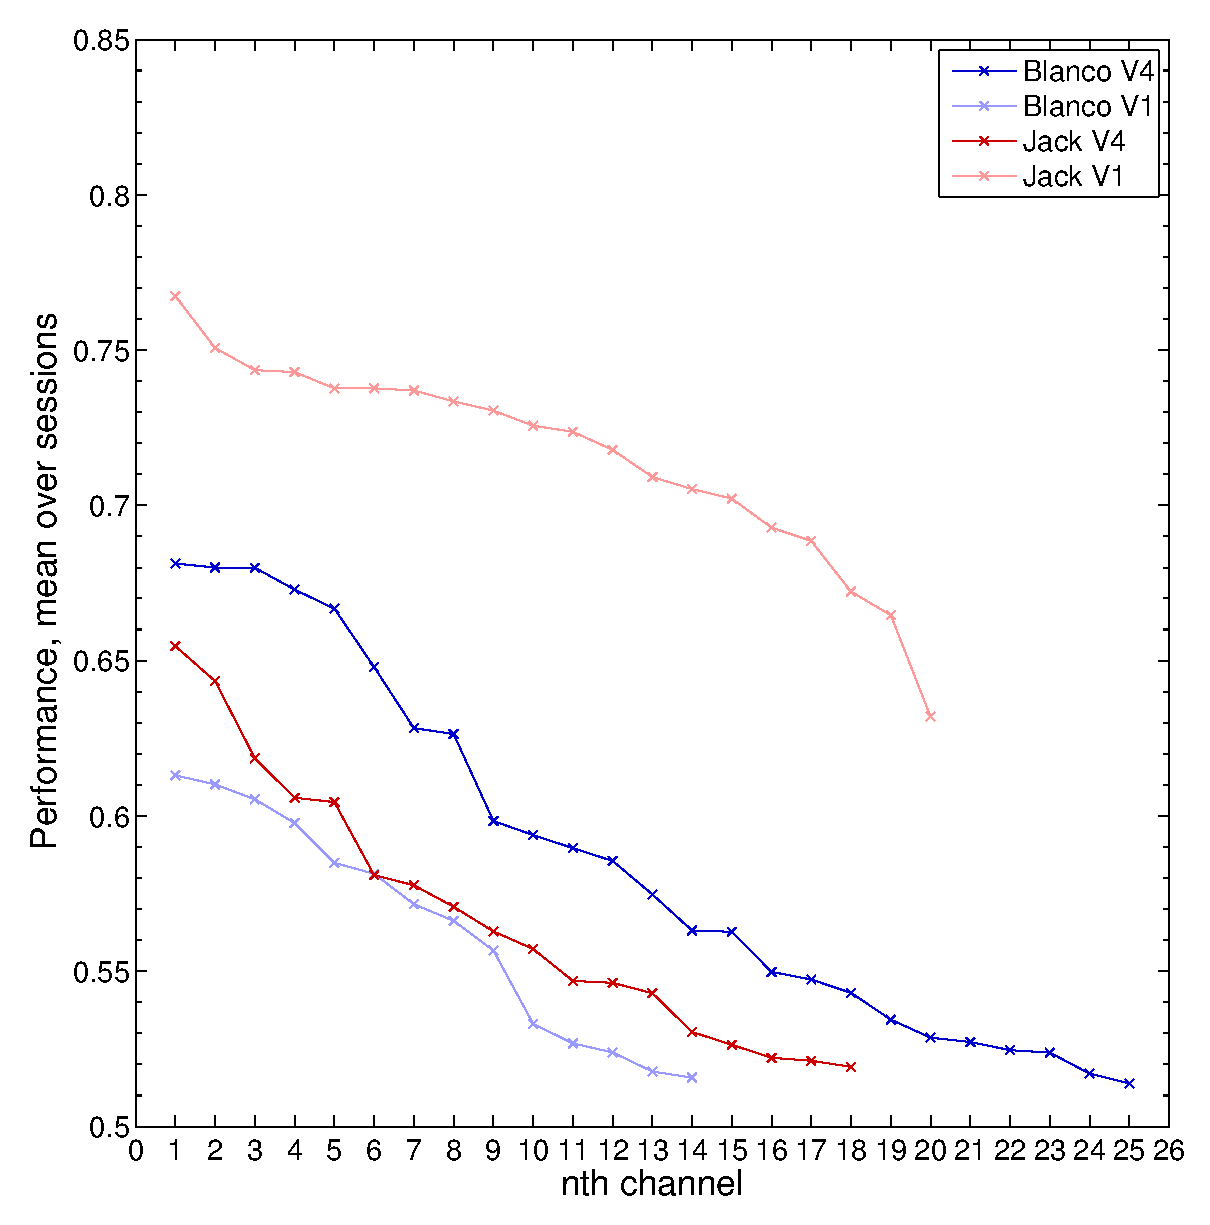
\includegraphics[width=\linewidth]{%
% % ./figs/decoding/2FC_singles.eps}
% %     \end{subfigure}
% %     ~~
% %     \begin{subfigure}[b]{0.5\linewidth}
% %         \centering
% %         \caption{}
% %         \label{fig:dec_nbest}
% %         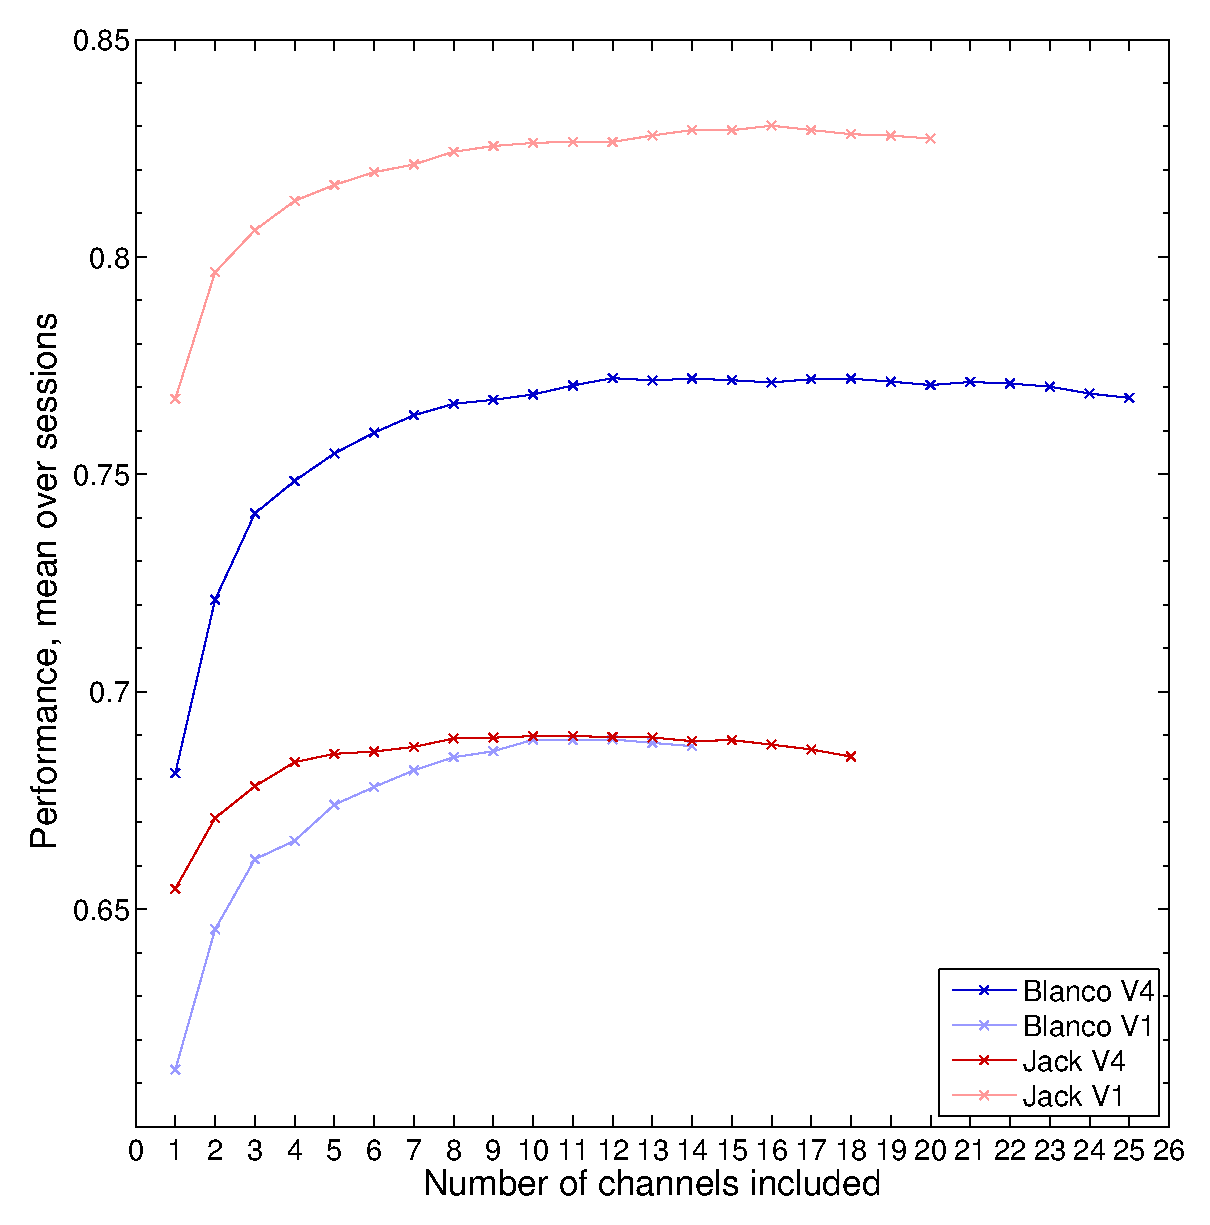
\includegraphics[width=\linewidth]{%
% % ./figs/decoding/2FC_nbest_all.eps}
% %     \end{subfigure}
% %     \caption{
% % \protect\subref{fig:dec_singles}: Distribution of decoder performance based on spike rate for individual channels, sorted by performance.
% % \protect\subref{fig:dec_nbest}: Decoding performance versus number of channels included in spiking data. Channels were added one at a time, chosen so they maximise the decoder performance for that number of channels whilst keeping all the channels which had come before.
% % }
% %     \label{fig:dec_n}
% % \end{figure}

For each of the datasets, the performance decreases as the last 3 channels are added (Fig.~\ref{fig:dec_nbest}). I speculate that this is because these channels only contain redundant information, and the increase in dimensionality decreases the quality of the classifier selected from the finite training data available.


% % \begin{figure}[htbp]
% %     \begin{subfigure}[b]{0.5\linewidth}
% %         \centering
% %         \caption{}
% %         \label{fig:dec_b4_allp}
% % 	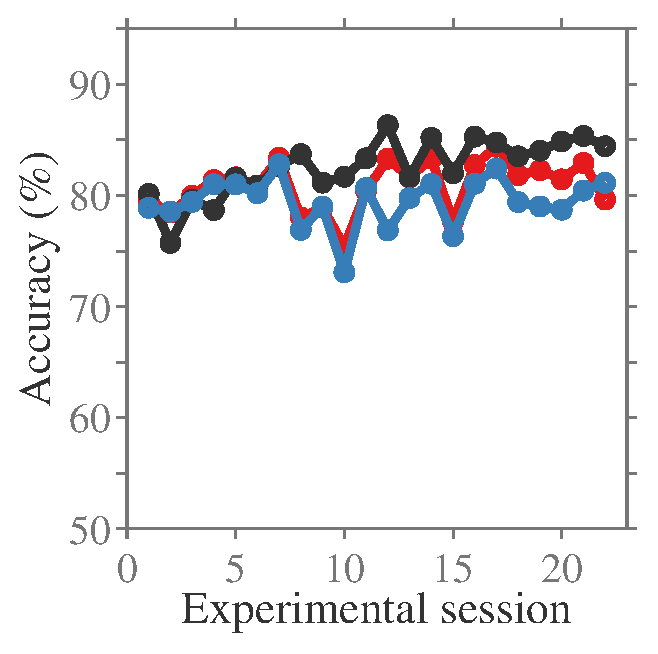
\includegraphics[width=\linewidth]{./figs/decoding/perf_v4_blanco.eps}
% %     \end{subfigure}
% %     ~~
% %     \begin{subfigure}[b]{0.5\linewidth}
% %         \centering
% %         \caption{}
% %         \label{fig:dec_j4_allp}
% % 	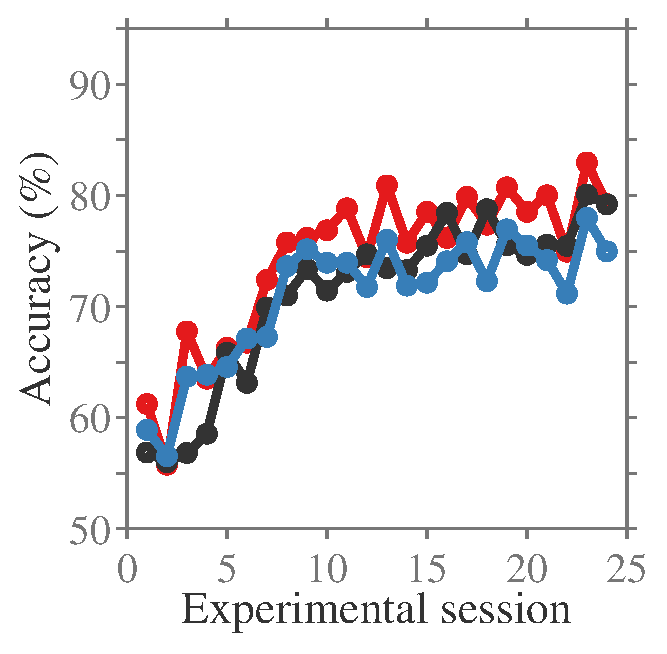
\includegraphics[width=\linewidth]{./figs/decoding/perf_v4_jack.eps}
% %     \end{subfigure}
% %     \caption{%
% %     Decoding analysis for V4. Performance of behavioural and decoding predictors by session, averaged across all conditions.
% %     Left panels: Blanco. Right: Jack.
% % 	Along the x-axis, `Session' is the animal's unique session ID, which increments by one for every day of training.
% %     On the y-axis, `proportion correct' is the proportion of trials for which the response is the same as the target.
% %     This is presented for behavioural performance (black), decoder performance (blue), and decoder performance when trials are shuffled, destroying noise correlations (red; see text).
% % }
% %     \label{fig:dec_all_v4}
% % \end{figure}

% % \begin{figure}[htbp]
% %     \begin{subfigure}[b]{0.5\linewidth}
% %         \centering
% %         \caption{}
% %         \label{fig:dec_b1_allp}
% % 	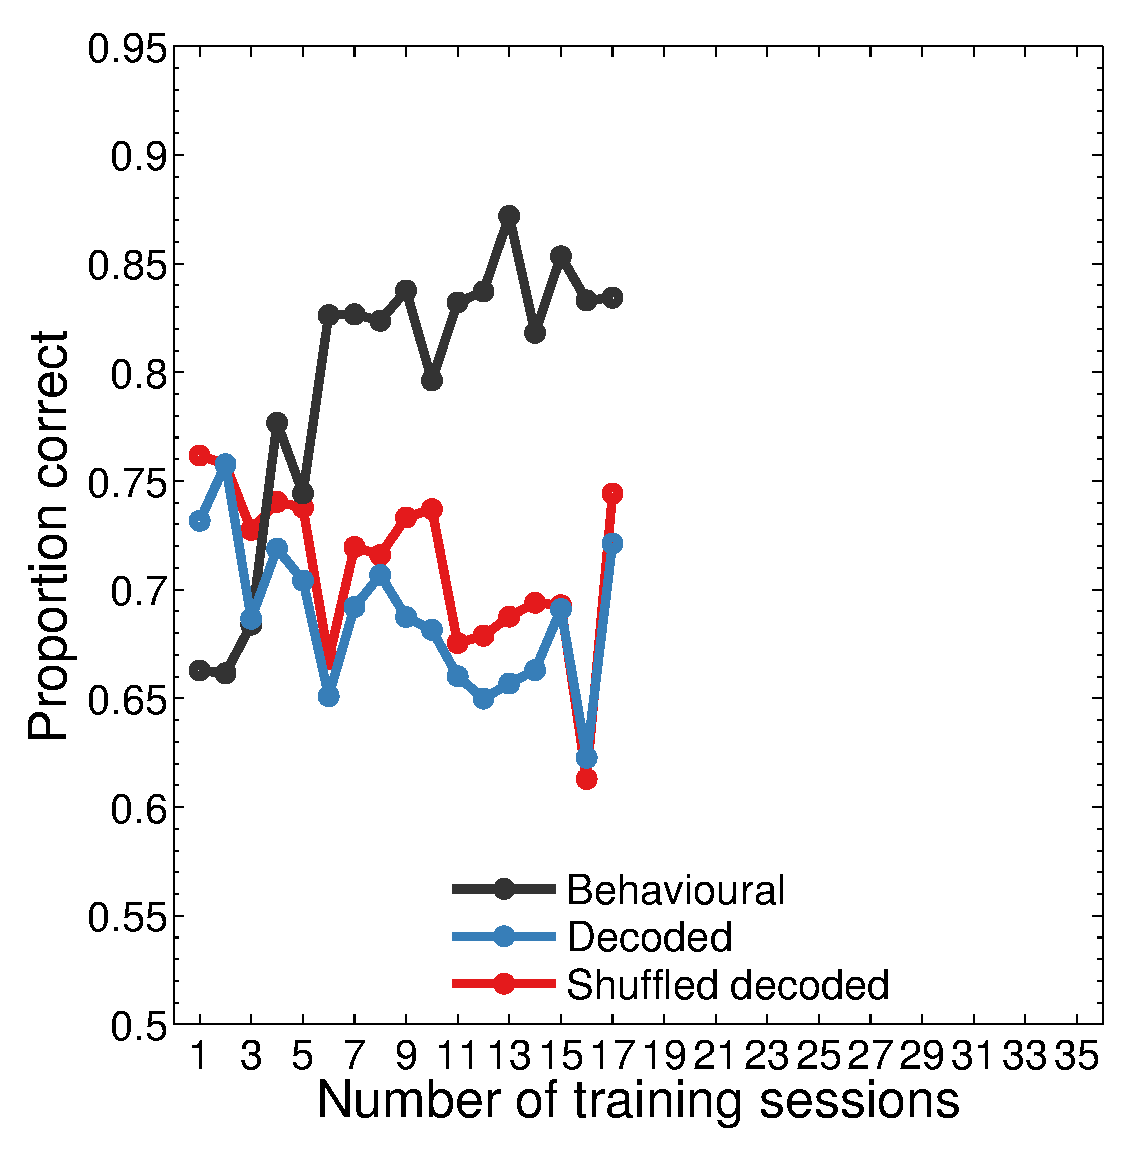
\includegraphics[width=\linewidth]{./figs/decoding/perf_v1_blanco.eps}
% %     \end{subfigure}
% %     ~~
% %     \begin{subfigure}[b]{0.5\linewidth}
% %         \centering
% %         \caption{}
% %         \label{fig:dec_j1_allp}
% % 	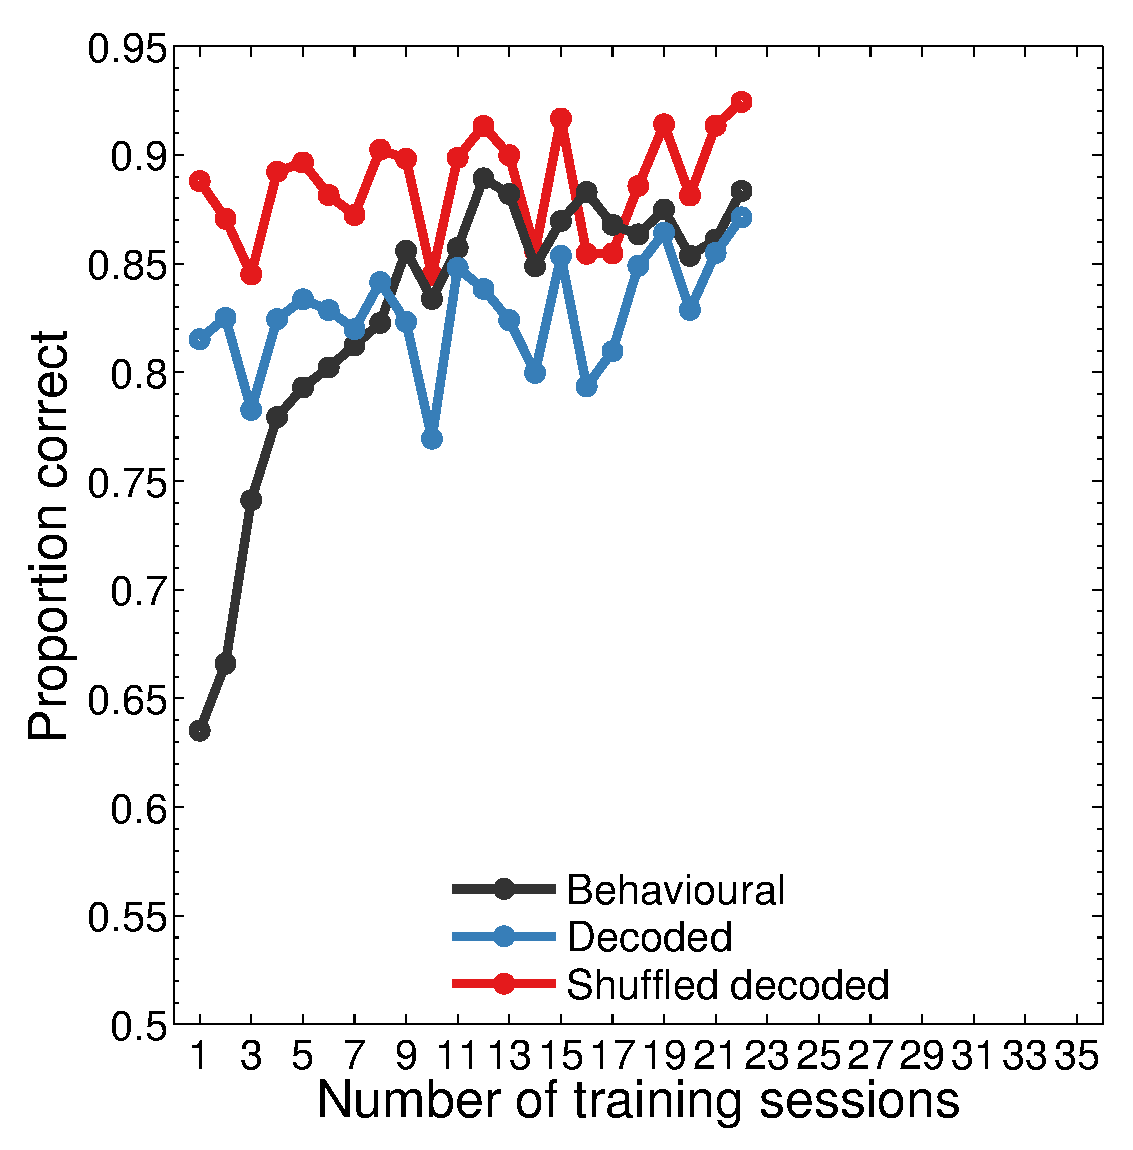
\includegraphics[width=\linewidth]{./figs/decoding/perf_v1_jack.eps}
% %     \end{subfigure}
% %     \caption{%
% %     Decoding analysis for V1. Performance of behavioural and decoding predictors by session, averaged across all conditions.
% %     Left panels: Blanco. Right: Jack.
% % 	Along the x-axis, `Session' is the animal's unique session ID, which increments by one for every day of training.
% %     On the y-axis, `proportion correct' is the proportion of trials for which the response is the same as the target.
% %     This is presented for behavioural performance (black), decoder performance (blue), and decoder performance when trials are shuffled, destroying noise correlations (red; see text).
% % }
% %     \label{fig:dec_all_v1}
% % \end{figure}



For Jack V4, the trend in increase for behavioural performance is well matched by the change in performance of the decoder (Fig.~\ref{fig:dec_j4_allp}, blue and red lines). In contrast to this, for Blanco V4 we see the decoding performance is steady despite training, although it should be noted that the increase in behavioural performance was not so large for this animal.

For Jack V1, there is a small gradual increase in decoder performance throughout training, though the increase does not match the timescales and rate of the increase in behavioural performance which is a much sharper transition. Results for Jack V1 could be interpreted as indicating that no further improvements can be obtained from changes in V1, and the behavioural performance is limited by the performance of the decoder.
For Blanco V1, there is a decrease in decoder in performance despite the increase in behavioural performance (Fig.~\ref{fig:dec_b1_allp}, blue and red lines respectively). 

Shuffling the trials to destroy any noise correlations provides an improvement in performance for the data from Jack, indicating that noise correlations are detrimental to the successful decoding of stimuli. However, there is no significant difference in decoder performance before and after shuffling for Blanco datasets, which suggests noise correlations have no impact on decoding the contrast of stimuli using firing rate data from a population of neurons.
For Jack V1, the benifit from shuffling seems to be reduced with training; the shuffled decoding performance is reasonably steady throughout training whilst the decoder with noise correlations included increases in performance, closing the gap.

% \marginnote{It might well be better to plot, for each area, the performances for both animals on the same plot and the expected vs observed behavioural agreement for both animals on a seperate plot.}


% % \begin{figure}[htbp]
% %     \begin{subfigure}[b]{0.5\linewidth}
% %         \centering
% %         \caption{}
% %         \label{fig:decag_b4_allp}
% % 	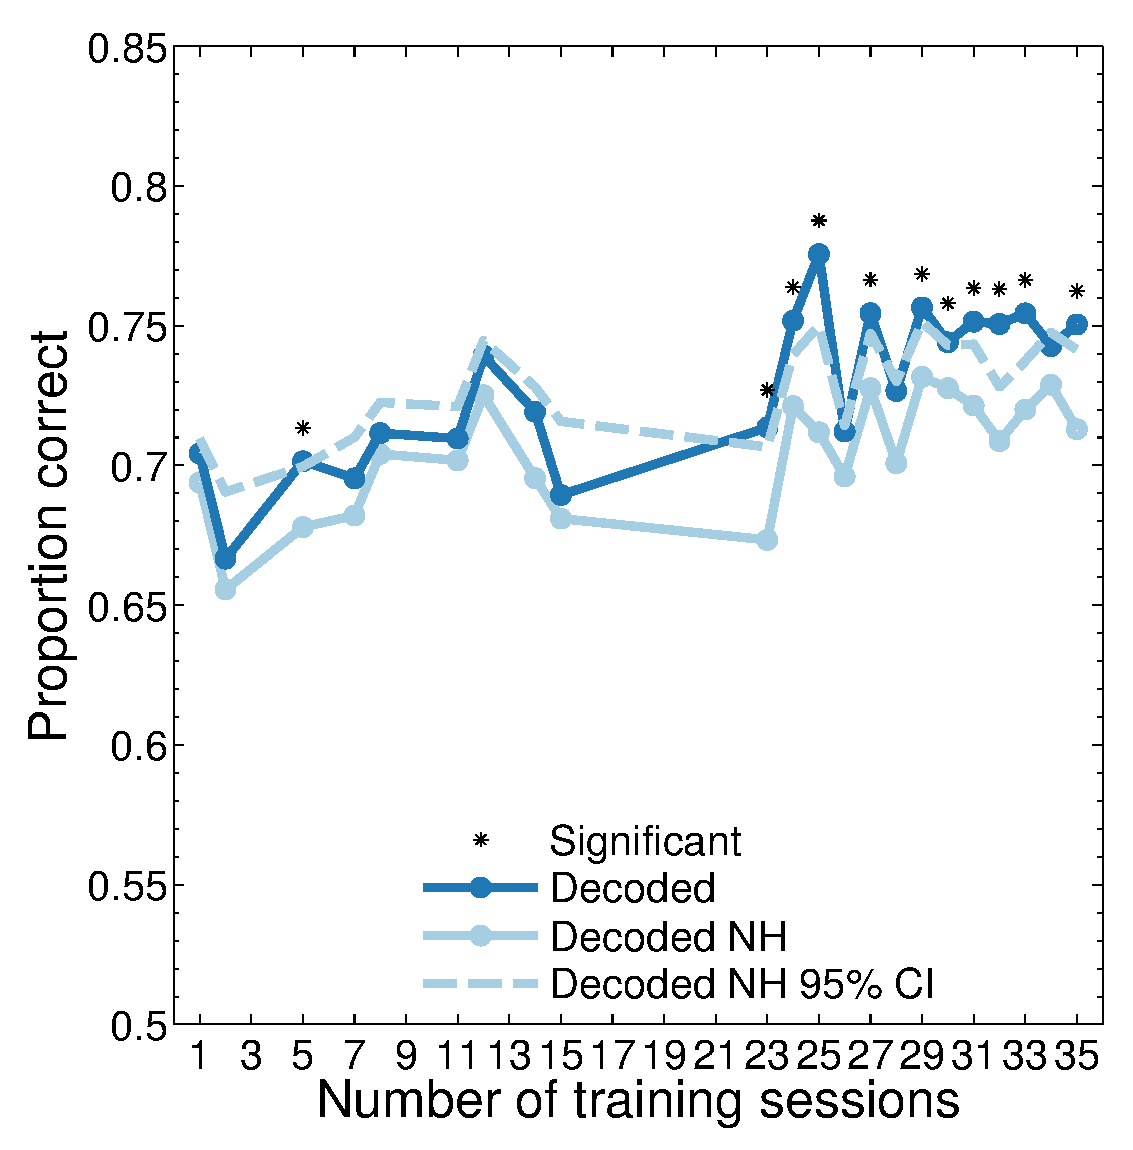
\includegraphics[width=\linewidth]{./figs/decoding/agree_v4_blanco.eps}
% %     \end{subfigure}
% %     ~~
% %     \begin{subfigure}[b]{0.5\linewidth}
% %         \centering
% %         \caption{}
% %         \label{fig:decag_j4_allp}
% % 	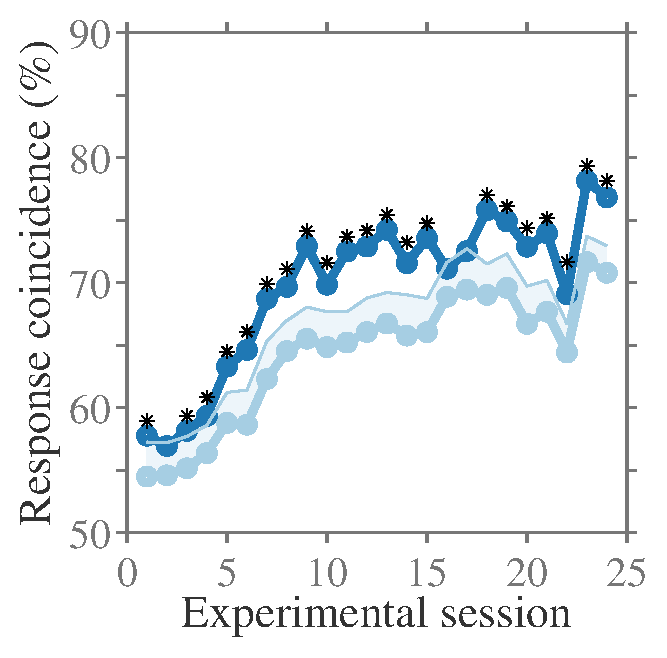
\includegraphics[width=\linewidth]{./figs/decoding/agree_v4_jack.eps}
% %     \end{subfigure}
% %     \caption{%
% %     Decoding analysis for V4. Trial-to-trial agreement between behavioural and decoding predictors.
% %     Left panels: Blanco. Right: Jack.
% % 	Along the x-axis, `Session' is the animal's unique session ID, which increments by one for every day of training.
% %     On the y-axis is the proportion of trials for which the response is the same as the behavioural response.
% %     The agreement between behaviour and decoding (unshuffled only) is presented alongside the null hypothesis of completely independent binomial distributions. The dashed line indicates the 95\% confidence interval of the null hypothesis.
% % }
% %     \label{fig:decag_all_v4}
% % \end{figure}

% % \begin{figure}[htbp]
% %     \begin{subfigure}[b]{0.5\linewidth}
% %         \centering
% %         \caption{}
% %         \label{fig:decag_b1_allp}
% % 	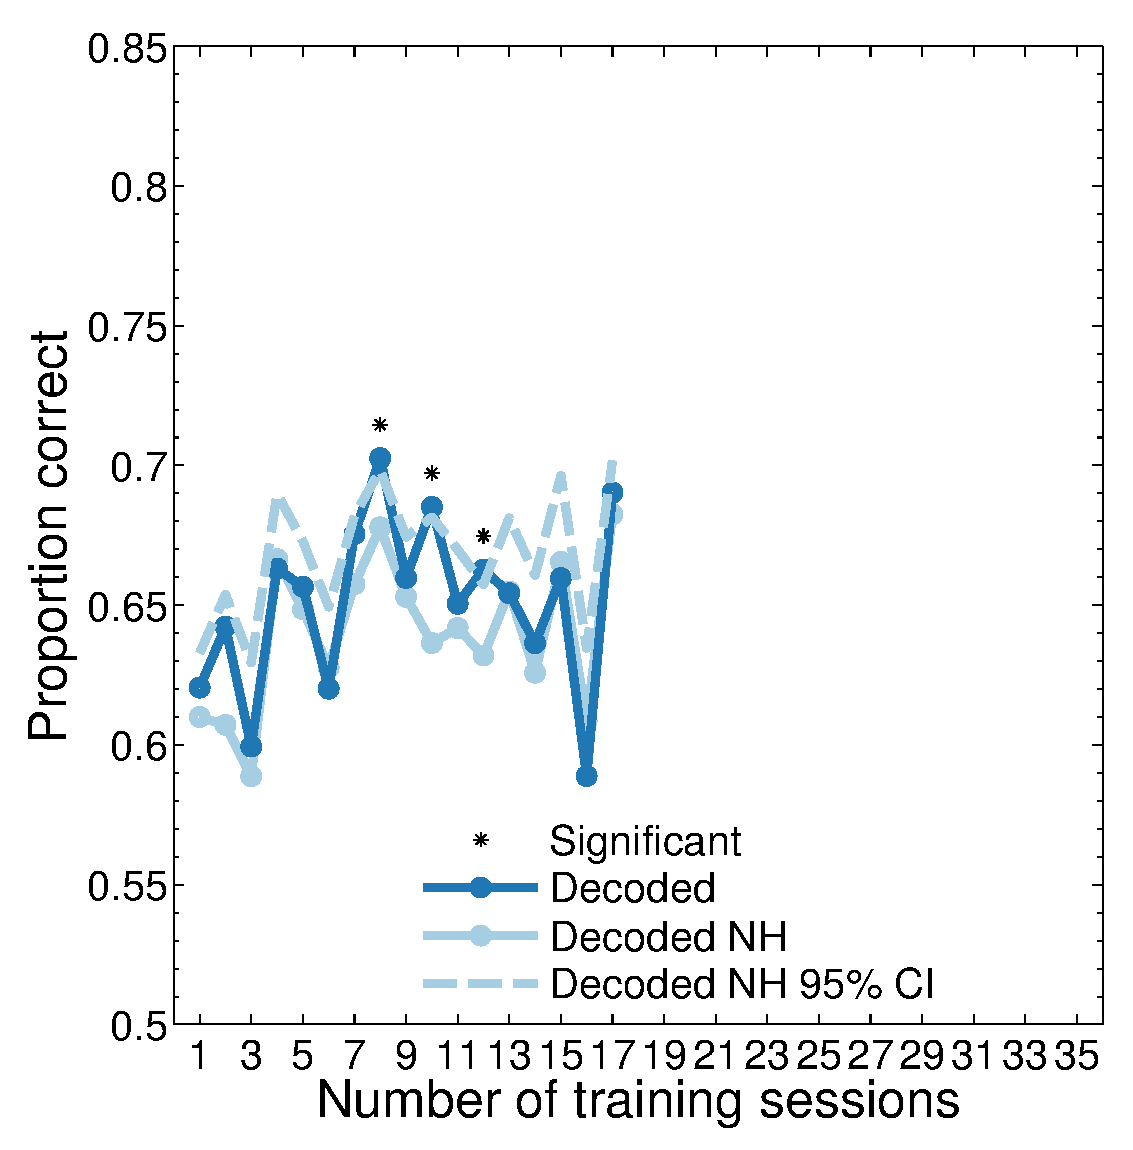
\includegraphics[width=\linewidth]{./figs/decoding/agree_v1_blanco.eps}
% %     \end{subfigure}
% %     ~~
% %     \begin{subfigure}[b]{0.5\linewidth}
% %         \centering
% %         \caption{}
% %         \label{fig:decag_j1_allp}
% % 	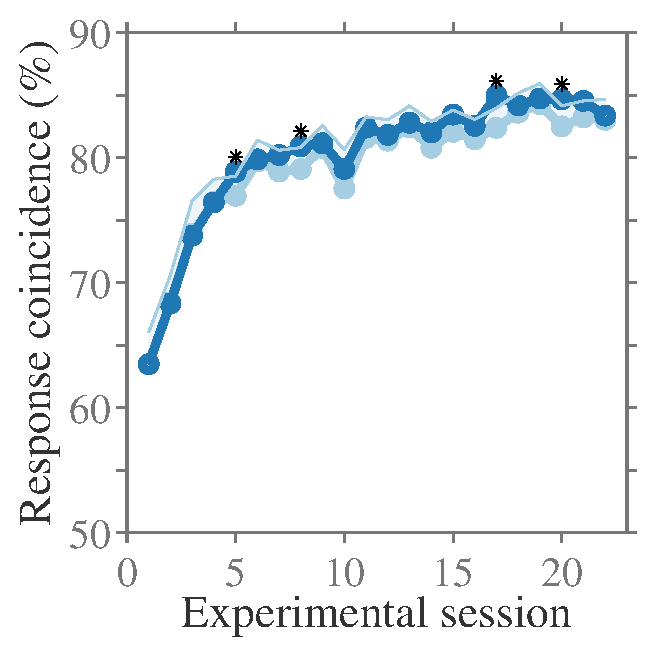
\includegraphics[width=\linewidth]{./figs/decoding/agree_v1_jack.eps}
% %     \end{subfigure}
% %     \caption{%
% %     Decoding analysis for V1. Trial-to-trial agreement between behavioural and decoding predictors.
% %     Left panels: Blanco. Right: Jack.
% % 	Along the x-axis, `Session' is the animal's unique session ID, which increments by one for every day of training.
% %     On the y-axis is the proportion of trials for which the response is the same as the behavioural response.
% %     The agreement between behaviour and decoding (unshuffled only) is presented alongside the null hypothesis of completely independent binomial distributions. The dashed line indicates the 95\% confidence interval of the null hypothesis.
% % }
% %     \label{fig:decag_all_v1}
% % \end{figure}


With regards to the behavioural and decoding response agreement, we find there is no consistent significant deviation from the null hypothesis for V1 data. There are a couple of sessions where unshuffled agreement is above the boundary for significance for each of the animals, but this is not a consistent effect. The agreement between shuffled decoding and behaviour does not deviate from the corresponding null hypothesis. This shows that the shuffled is higher than the unshuffled decoding agreement only because the shuffled decoder is more accurate at matching the target response.

For V4, we see that the agreement does not deviate significantly from the null hypothesis for earlier sessions, but after a cut off point all later sessions do (Blanco: all sessions before 321 are not, after 329 are significant; Jack: Before 28 are not, after 28 are significant). The effect is stronger for Jack, but present for both animals.
This indicates that the behavioural responses and the decoded responses based on the neural data were not notably correlated, but have become so with training.

Because the shuffled decoded responses are more accurate (with respect to the target response), they are predicted under the null hypothesis to be in better agreement with the behavioural responses. However we observe these are in worse agreement than the unshuffled decoding, and do not deviate from the corresponding NH line.

A more detailed breakdown of these results with subsets of the 14 conditions is given in Figs.~\ref{fig:dec_detail_b1} and \ref{fig:dec_detail_j4}.
Comparing Figs.~\ref{fig:dec_b4_6easy_a} and \ref{fig:dec_j4_6easy_a} with Figs.~\ref{fig:dec_b4_6hard_a} and \ref{fig:dec_j4_6hard_a}, we can see that the decoding responses for the easier conditions fit the null hypothesis model, whilst the more challenging conditions do not and have a statistically significant agreement with the animal behaviour.




% ----------------------------------------------
\clearpage
\subsection{Noise correlations}
% ----------------------------------------------

For both V1 and V4, the average noise correlation between pairs of channels seem to remain stable for Blanco and decrease by a small margin for Jack (see Fig.~\ref{fig:noise_r_all}). The increase in noise correlation for Blanco V1 for the last two sessions (session numbers 358 and 359) is due to a decline in data quality and an increase in noise from artificial sources. There is a large amount of variance in the noise correlations for different pairs, so the decline in mean correlation for Jack does not seem very large considering the amount of variance.


% % \begin{figure}[htb]
% %     \begin{subfigure}[b]{0.5\linewidth}
% %         \centering
% %         \caption{}
% %         \label{fig:noise_r_v1_all}
% % %         \includegraphics[width=\linewidth]{%
% % % ./rcoef_2013-04-09/rcoef_sess_meanpc_2013-04-09/png/rcoef_sess_meanpc_v1_both.png}
% % %        \includegraphics[width=\linewidth]{./figs/decoding/rcoef_sess_meanpc_v1_both}
% %         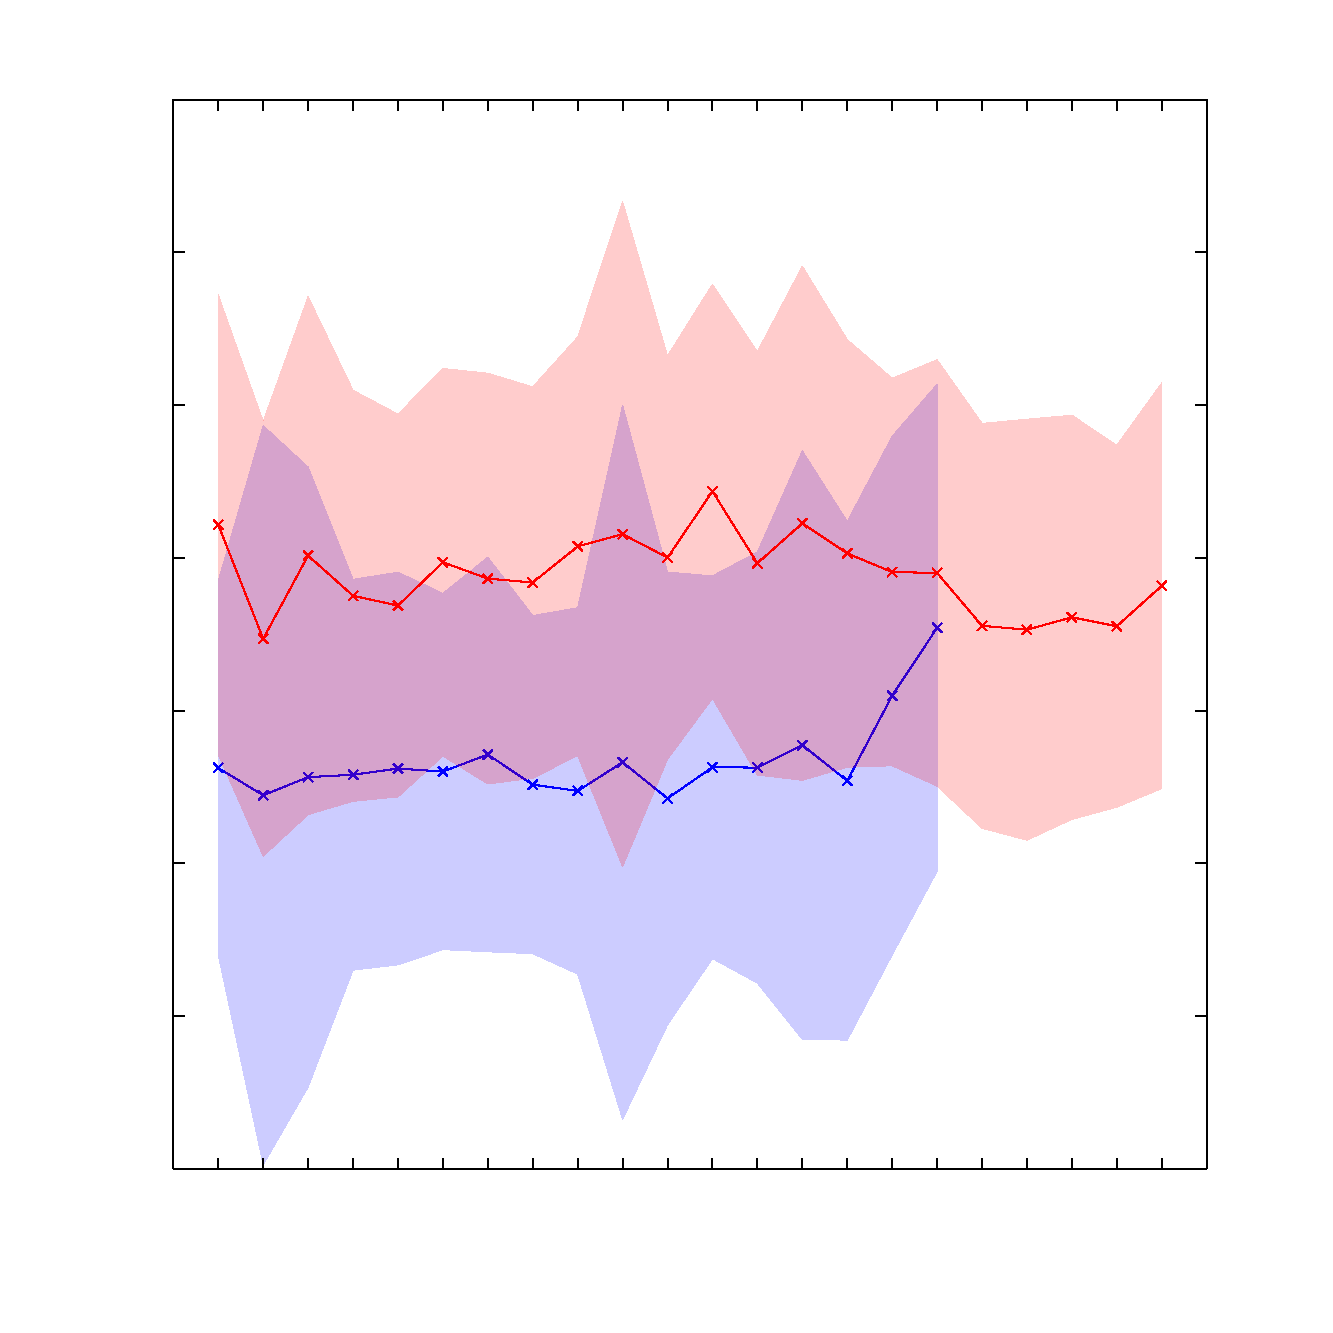
\includegraphics[width=\linewidth]{./figs/decoding/rcoef_sess_meanpc_v1_both.pdf}
% %     \end{subfigure}
% %     ~~
% %     \begin{subfigure}[b]{0.5\linewidth}
% %         \centering
% %         \caption{}
% %         \label{fig:noise_r_v4_all}
% % %         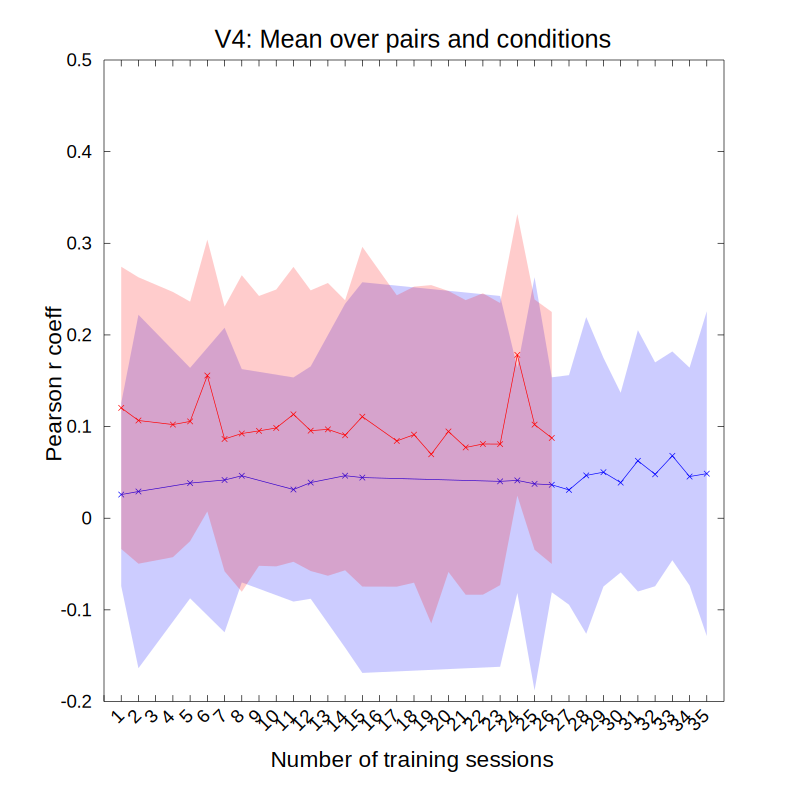
\includegraphics[width=\linewidth]{%
% % % ./rcoef_2013-04-09/rcoef_sess_meanpc_2013-04-09/png/rcoef_sess_meanpc_v4_both.png}
% %         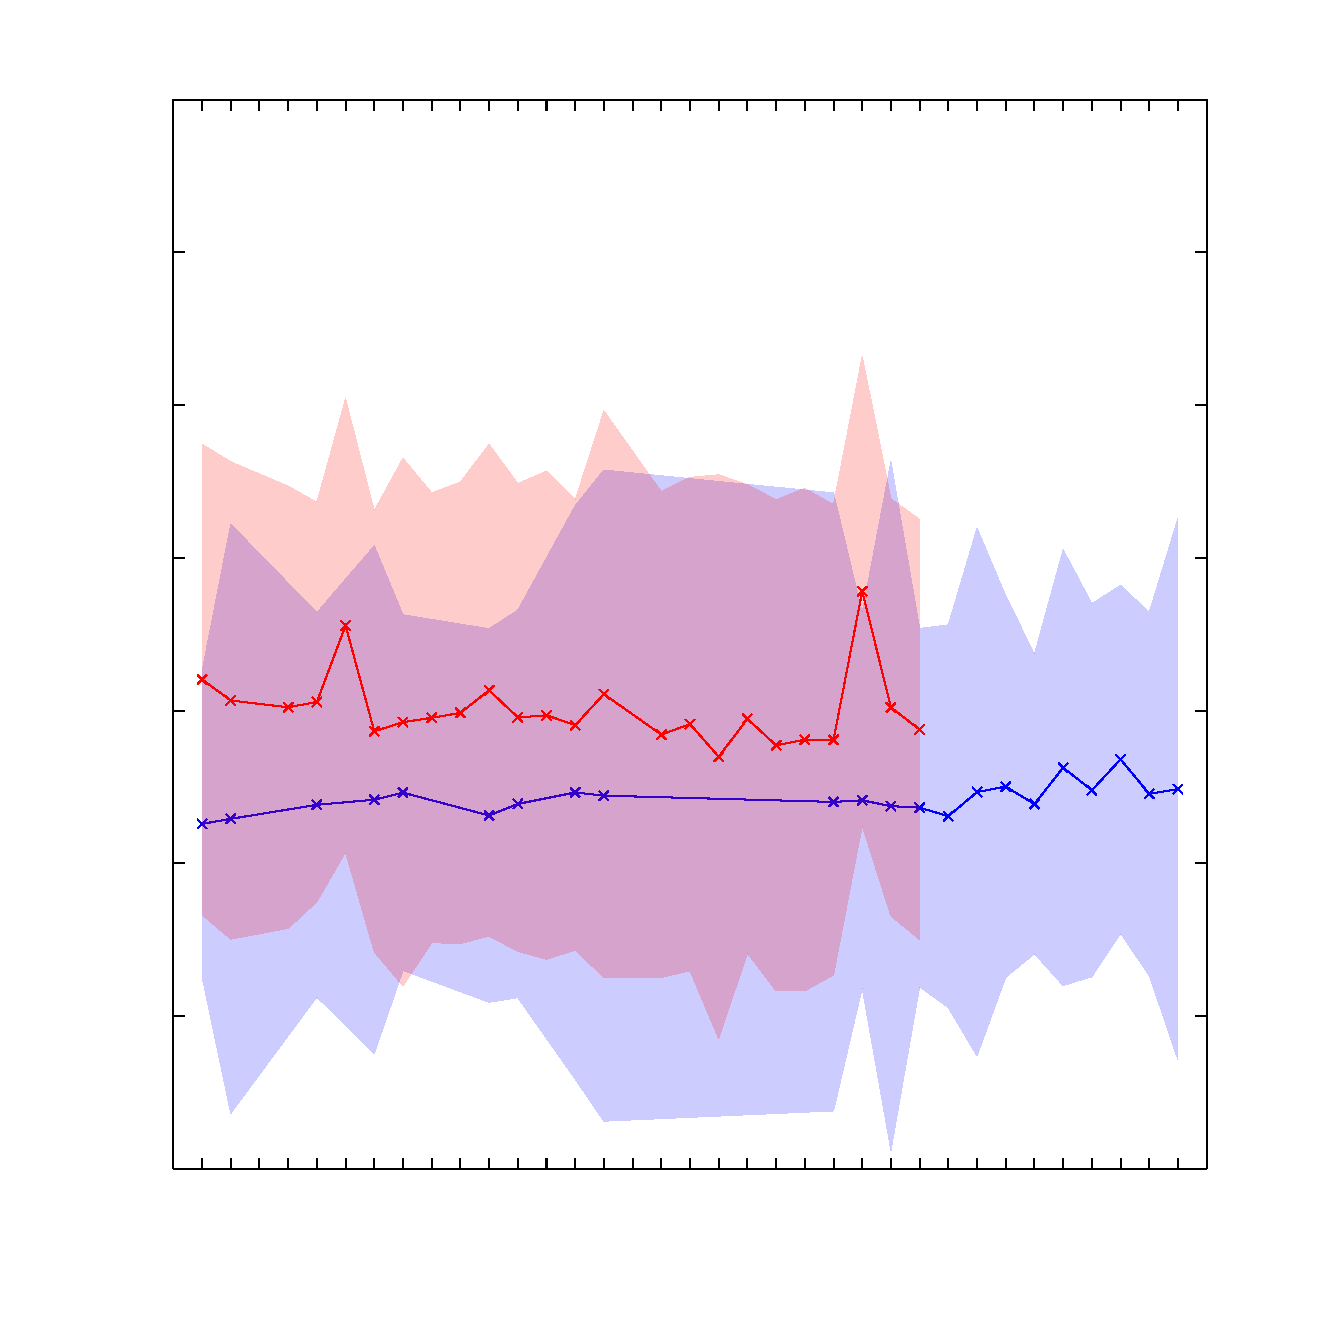
\includegraphics[width=\linewidth]{./figs/decoding/rcoef_sess_meanpc_v4_both.pdf}
% %     \end{subfigure}
% %     \caption{Change in noise correlations with learning.
% % \protect\subref{fig:noise_r_v1_all}:~V1.
% % \protect\subref{fig:noise_r_v4_all}:~V4.
% % Blue:~Blanco.
% % Red:~Jack.
% % On the x-axis, the number of sessions since the animal began training in the part of the visual field retinotopic to the recording site is shown.
% % Line: pearson r coefficient, averaged across the possible pairings between channels for each of the 14 trial conditions.
% % Shaded region indicates one standard deviation from mean.
% % }
% %     \label{fig:noise_r_all}
% % \end{figure}
% \marginnote{In Fig.~\ref{fig:noise_r_all} and \ref{fig:noise_r_hist}, the text is too small due to saving the figure with transparencies in PNG format; if I could get the SVG to load correctly, the text would be sized correctly.}

Fig.~\ref{fig:noise_r_hist} is intended to reproduce Figure 2C from \citet{Gu2011}, with the distribution of $r$ shown across pairs for one pre-training and one post-training session. These sessions were chosen from a restricted set of sessions which did not have problems with artificially high correlations from the motion artifact, and selected from this set such that they were as close to the start and end of the training period as possible. However, this selection was made before the set of trials was redacted as mentioned in \S\ref{sec:dec-meth-noise}, so the sessions selected could possibly be made further apart.

The data presented in Fig.~\ref{fig:noise_r_hist} shows that the distribution of noise correlation pairs does not move significantly for Blanco V1, which is contrasted by a clear decrease for Jack V1. It should be noted though that the distribution for Jack V1 begins higher than Blanco and decreases to a similar value as Blanco V1. For V4, there is an increase in mean noise correlation for Blanco and a decrease for Jack, though as Jack begins higher than Blanco the two do tend toward to one another.

Cherry-picking is a significant problem here, as there is sizable day-to-day variation in the noise correlation across the pairs. Choosing a session where there is more noise correlation than neighbouring sessions at the beginning of training and less at the end of training will give the impression that there is a more significant decrease in noise correlations. More effort should be made to counter inadvertently cherry-picking in the session selection, as Fig.~\ref{fig:noise_r_j1_pmc} indicates this may be one reason for such a sizable decrease in noise correlation for Jack V1.

% % \begin{figure}[htbp]
% %     \begin{subfigure}[b]{0.5\linewidth}
% %         \centering
% %         \caption{}
% %         \label{fig:noise_r_b1_hist}
% % %         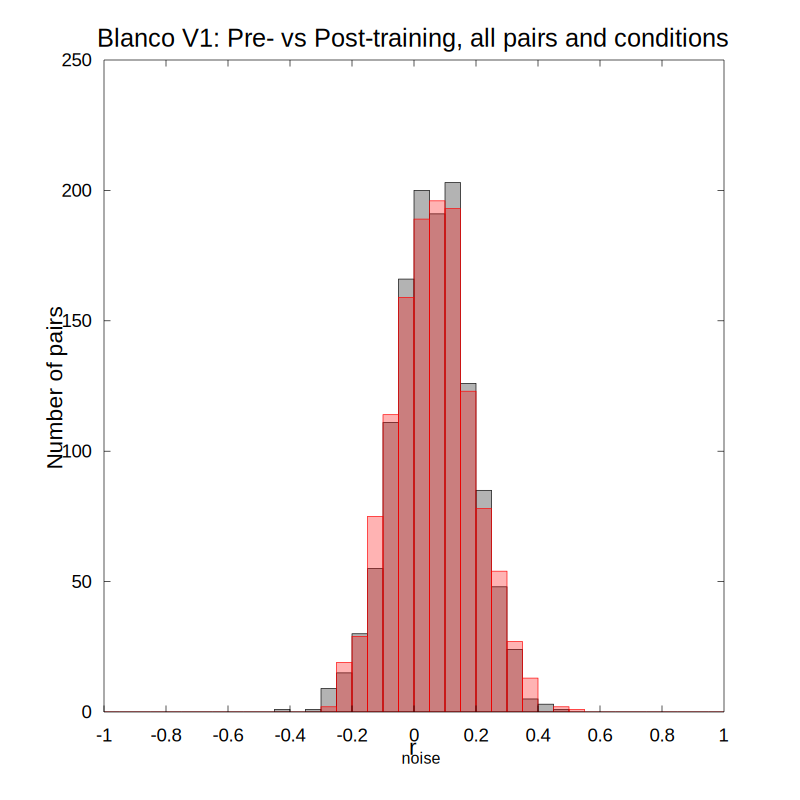
\includegraphics[width=\linewidth]{%
% % % ./rcoef_2013-03-25/rcoef_sess_histallover_2013-03-25/png/rcoef_sess_histallover_v1_blanco.png}
% %         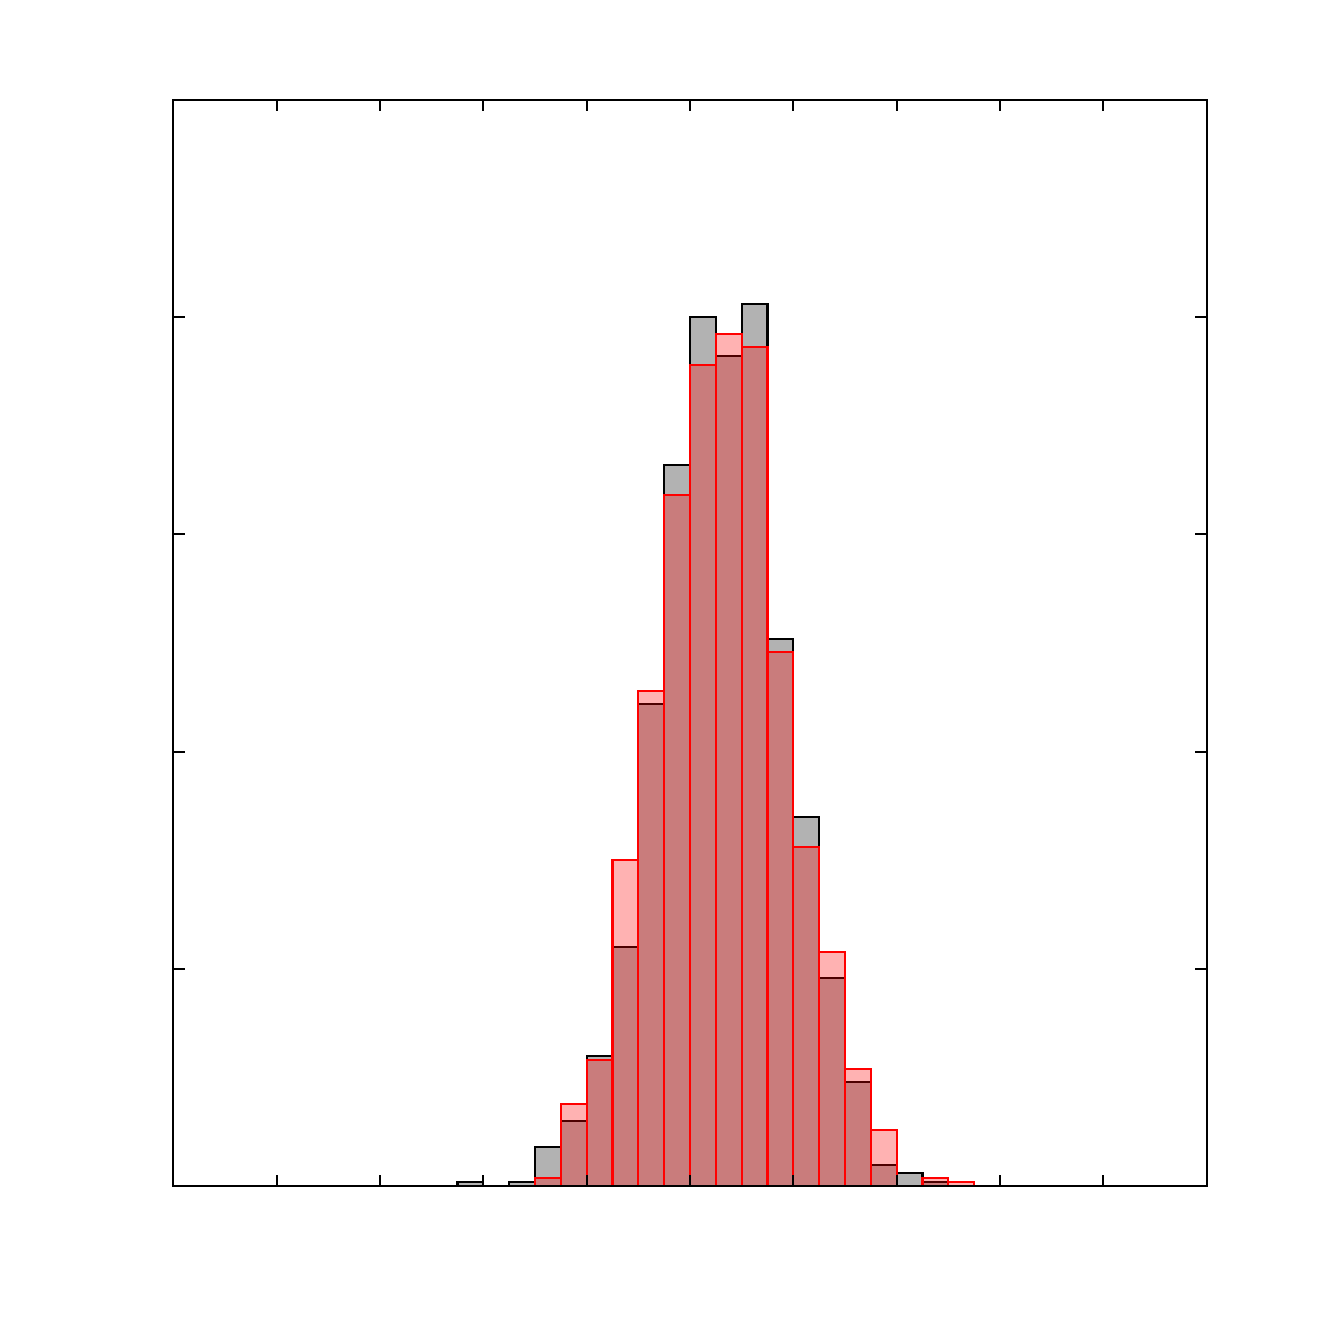
\includegraphics[width=\linewidth]{./figs/decoding/rcoef_sess_histallover_v1_blanco.pdf}
% %     \end{subfigure}
% %     ~~
% %     \begin{subfigure}[b]{0.5\linewidth}
% %         \centering
% %         \caption{}
% %         \label{fig:noise_r_j1_hist}
% % %         \includegraphics[width=\linewidth]{%
% % % ./rcoef_2013-03-25/rcoef_sess_histallover_2013-03-25/png/rcoef_sess_histallover_v1_jack.png}
% %         \includegraphics[width=\linewidth]{./figs/decoding/rcoef_sess_histallover_v1_jack.pdf}
% %     \end{subfigure}
% %     \\
% %     \begin{subfigure}[b]{0.5\linewidth}
% %         \centering
% %         \caption{}
% %         \label{fig:noise_r_b4_hist}
% % %         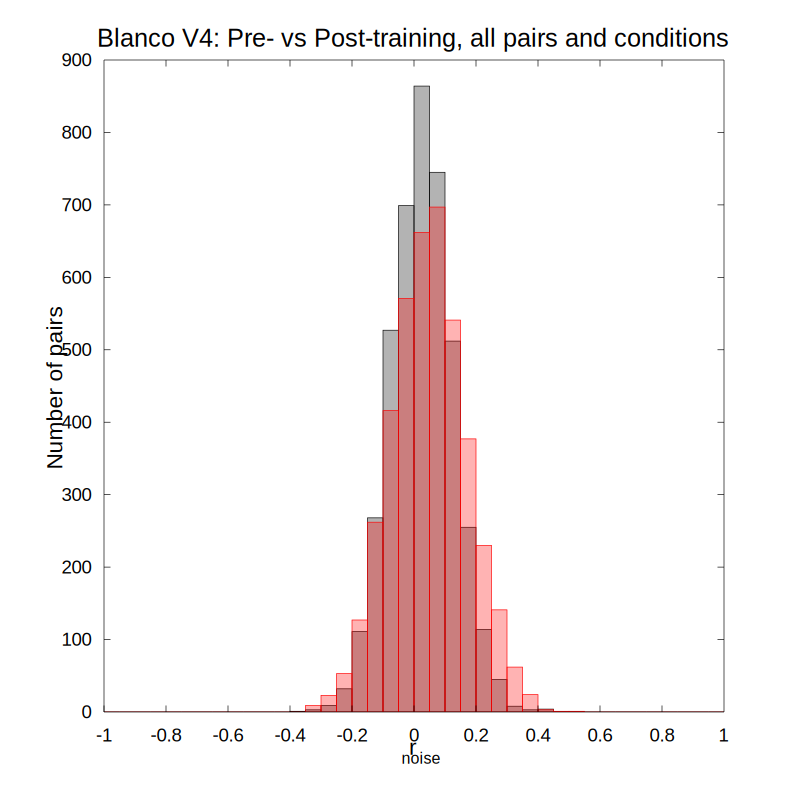
\includegraphics[width=\linewidth]{%
% % % ./rcoef_2013-03-25/rcoef_sess_histallover_2013-03-25/png/rcoef_sess_histallover_v4_blanco.png}
% %         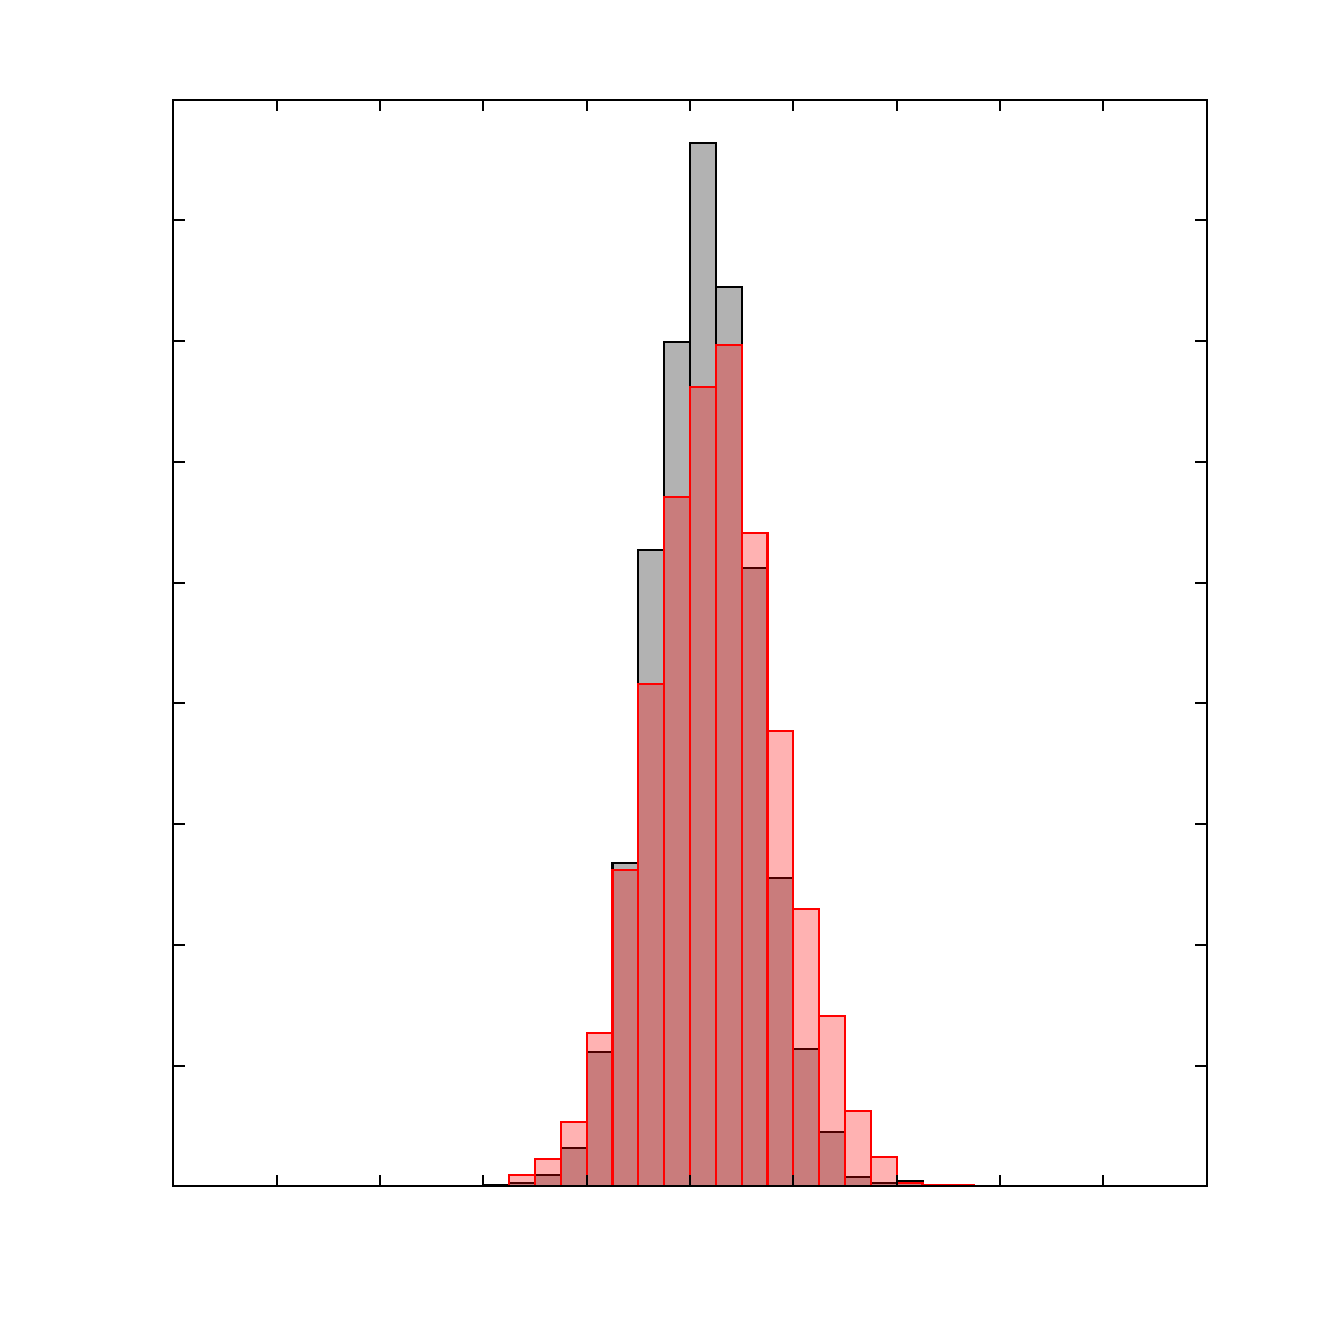
\includegraphics[width=\linewidth]{./figs/decoding/rcoef_sess_histallover_v4_blanco.pdf}
% %     \end{subfigure}
% %     ~~
% %     \begin{subfigure}[b]{0.5\linewidth}
% %         \centering
% %         \caption{}
% %         \label{fig:noise_r_j4_hist}
% % %         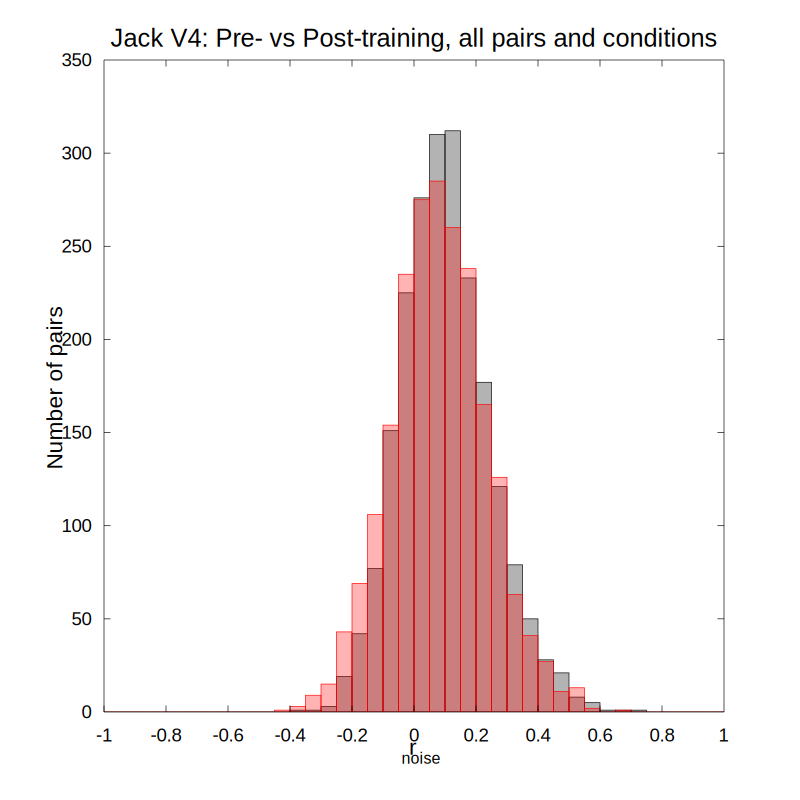
\includegraphics[width=\linewidth]{%
% % % ./rcoef_2013-03-25/rcoef_sess_histallover_2013-03-25/png/rcoef_sess_histallover_v4_jack.png}
% %         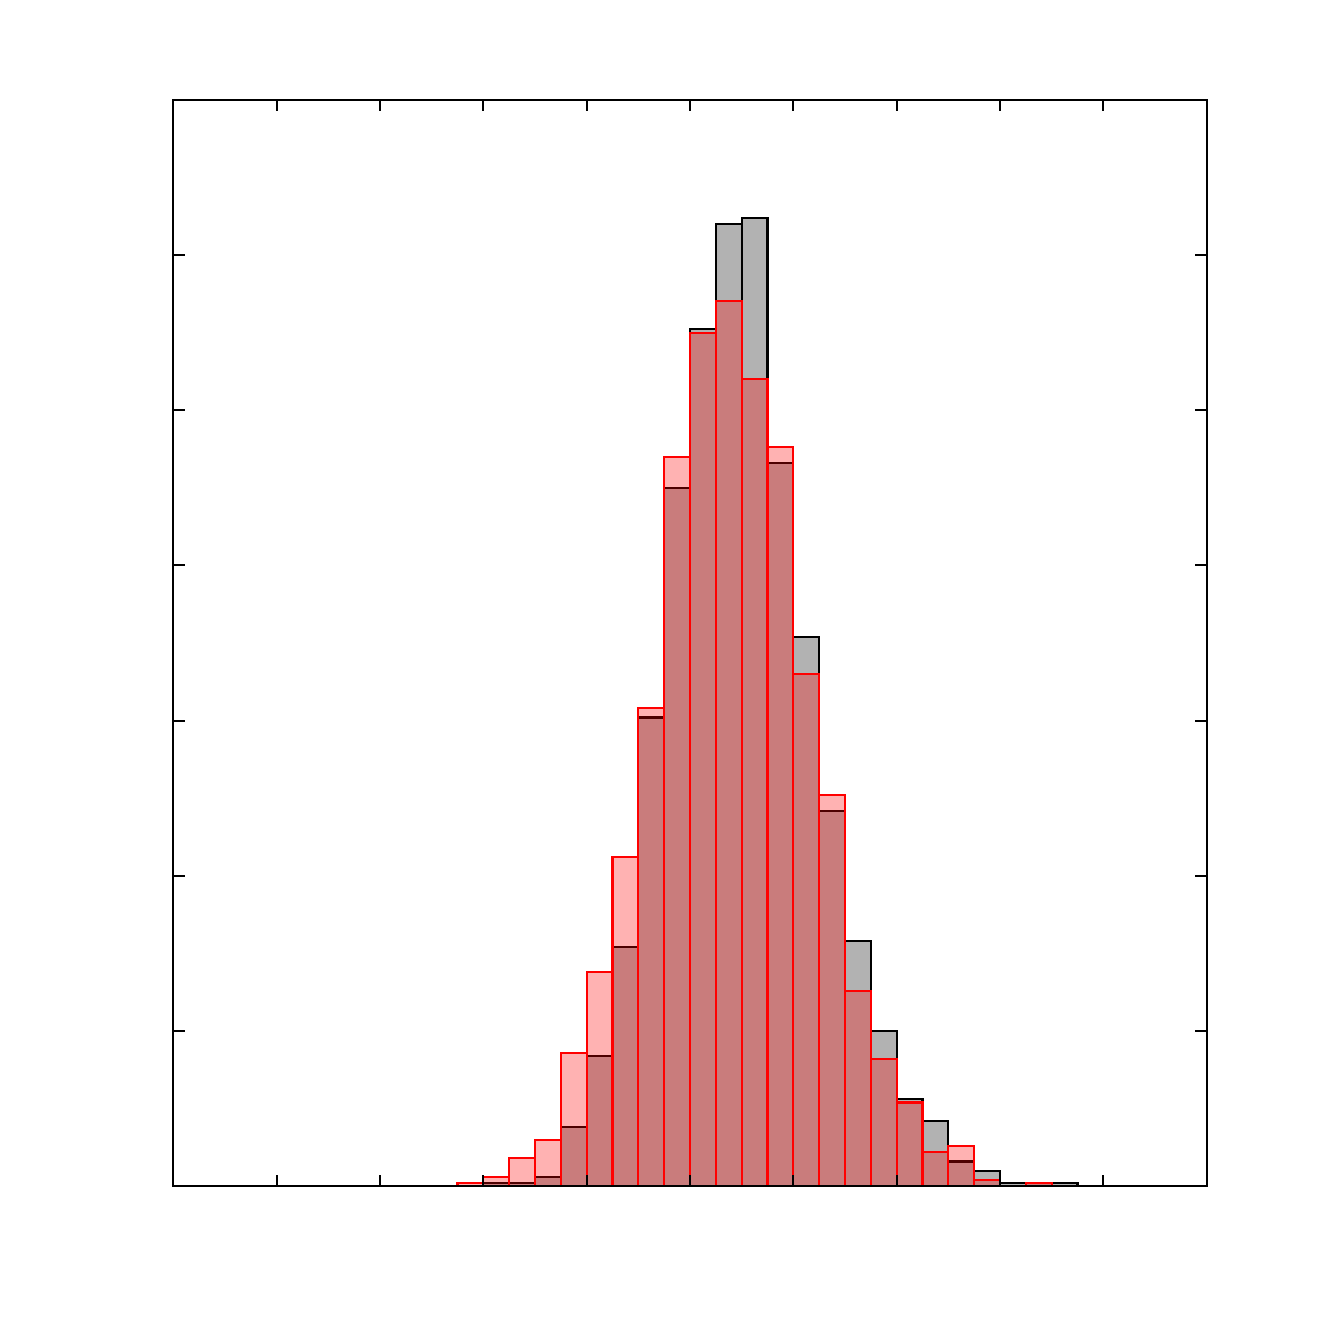
\includegraphics[width=\linewidth]{./figs/decoding/rcoef_sess_histallover_v4_jack.pdf}
% %     \end{subfigure}
% %     \caption{Distribution of the noise correlations for the pairings across all conditions.
% % Two sessions, one at the beginning of training (black) and one at the end of training (red) are shown for comparitive purposes.
% % \protect\subref{fig:noise_r_b1_hist}: Blanco V1; sessions 343 and 354.
% % \protect\subref{fig:noise_r_j1_hist}: Jack V1; sessions 51 and 71.
% % \protect\subref{fig:noise_r_b4_hist}: Blanco V4; sessions 307 and 338.
% % \protect\subref{fig:noise_r_j4_hist}: Jack V4; sessions 27 and 46.
% % }
% %     \label{fig:noise_r_hist}
% % \end{figure}


% Fig.~\ref{fig:noise_r_pmc} indicates that noise correlations are correlated for pairs across sessions.
A pairs of channels which have higher noise correlations in one session are likely to have higher noise correlation in other sessions. However, this effect is not present for Blanco V1, Fig.~\ref{fig:noise_r_b1_pmc}, and could suggest there is less session-to-session consistency for this dataset.

This figure provides an easy way of visually inspecting whether noise correlations are conserved, but does not allow us to quantify this.

% % \begin{figure}[htbp]
% %     \begin{subfigure}[b]{0.5\linewidth}
% %         \centering
% %         \caption{}
% %         \label{fig:noise_r_b1_pmc}
% %         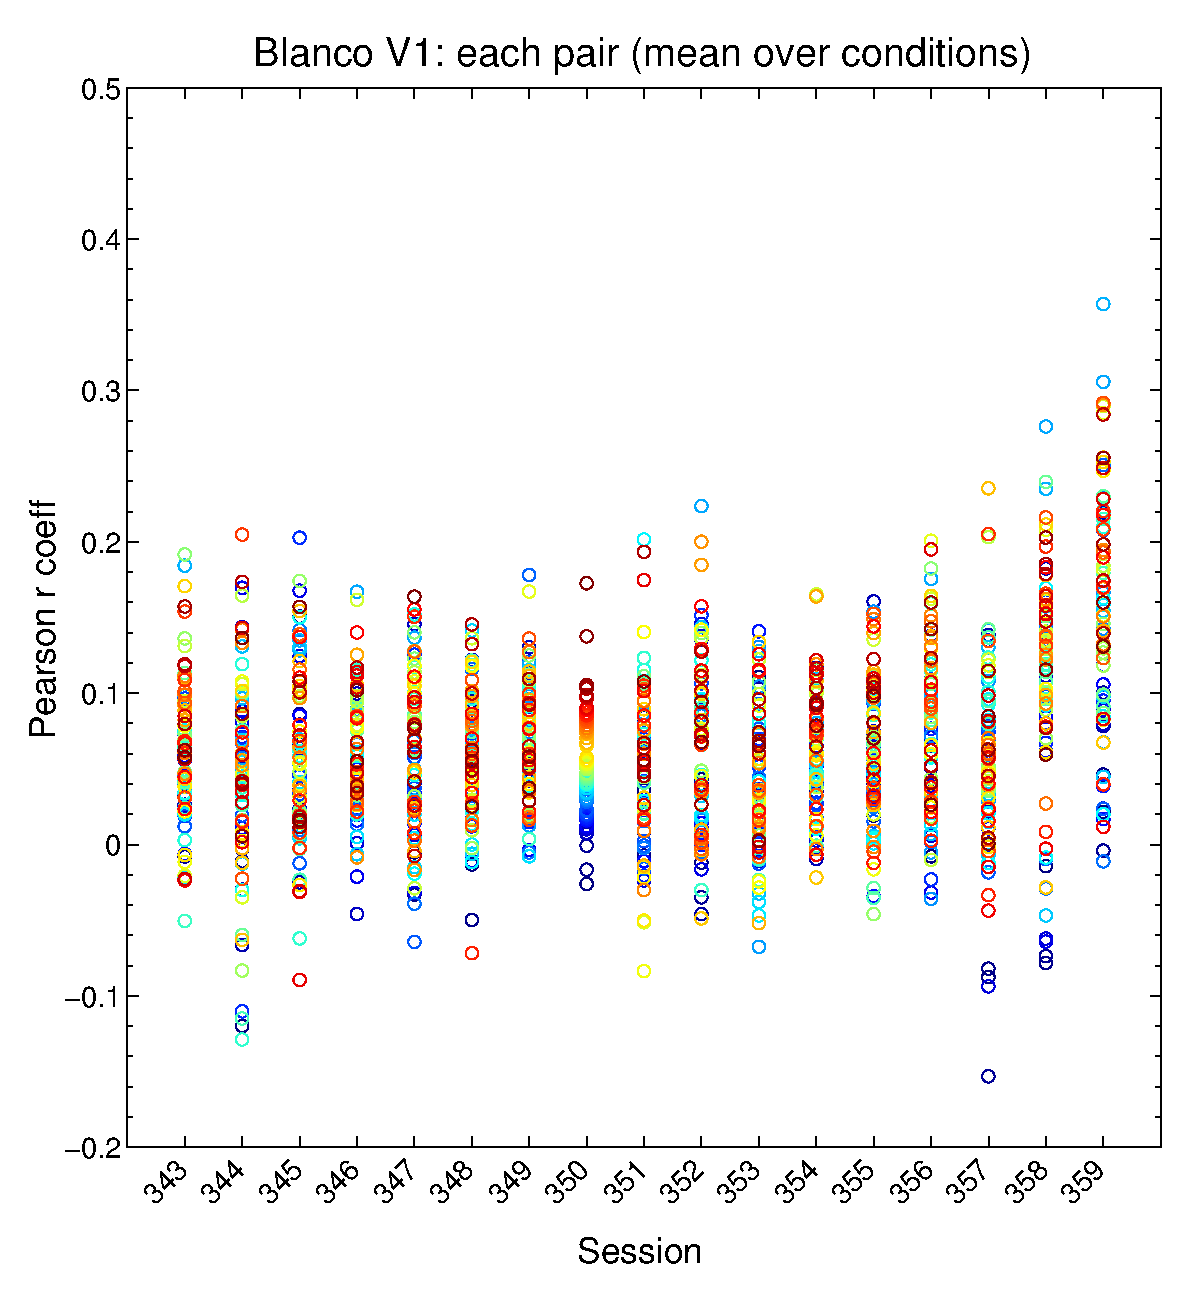
\includegraphics[width=\linewidth]{%
% % ./figs/decoding/rcoef_sess_pairsmeanc_v1_blanco.eps}
% %     \end{subfigure}
% %     ~~
% %     \begin{subfigure}[b]{0.5\linewidth}
% %         \centering
% %         \caption{}
% %         \label{fig:noise_r_j1_pmc}
% %         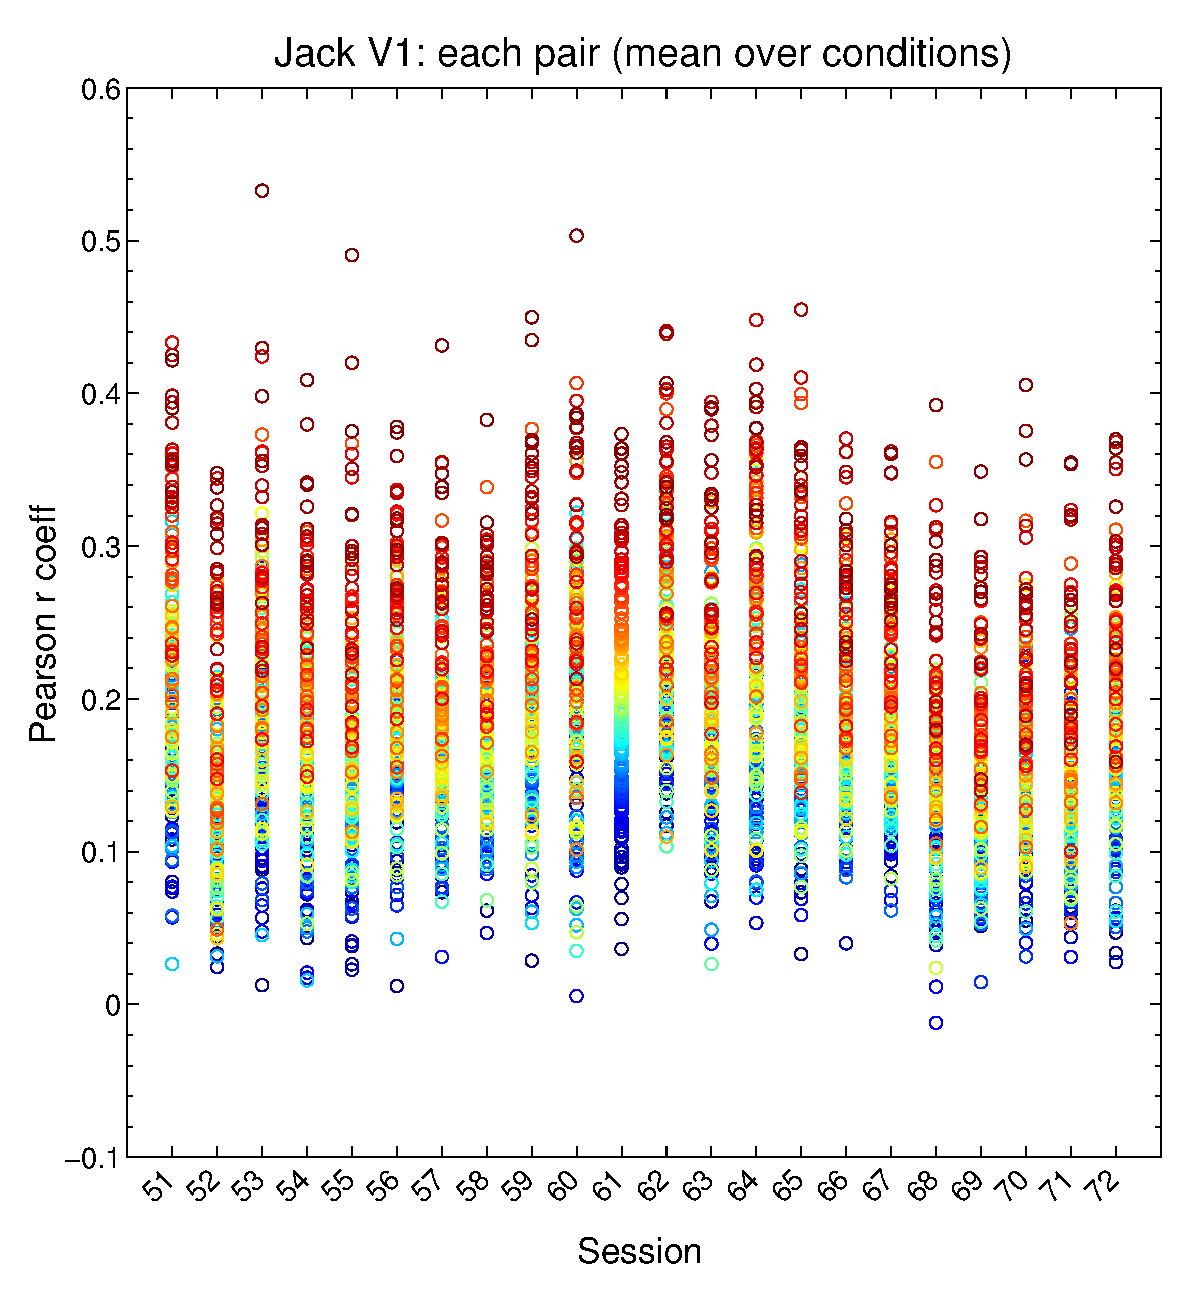
\includegraphics[width=\linewidth]{%
% % ./figs/decoding/rcoef_sess_pairsmeanc_v1_jack.eps}
% %     \end{subfigure}
% %     \\
% %     \begin{subfigure}[b]{0.5\linewidth}
% %         \centering
% %         \caption{}
% %         \label{fig:noise_r_b4_pmc}
% %         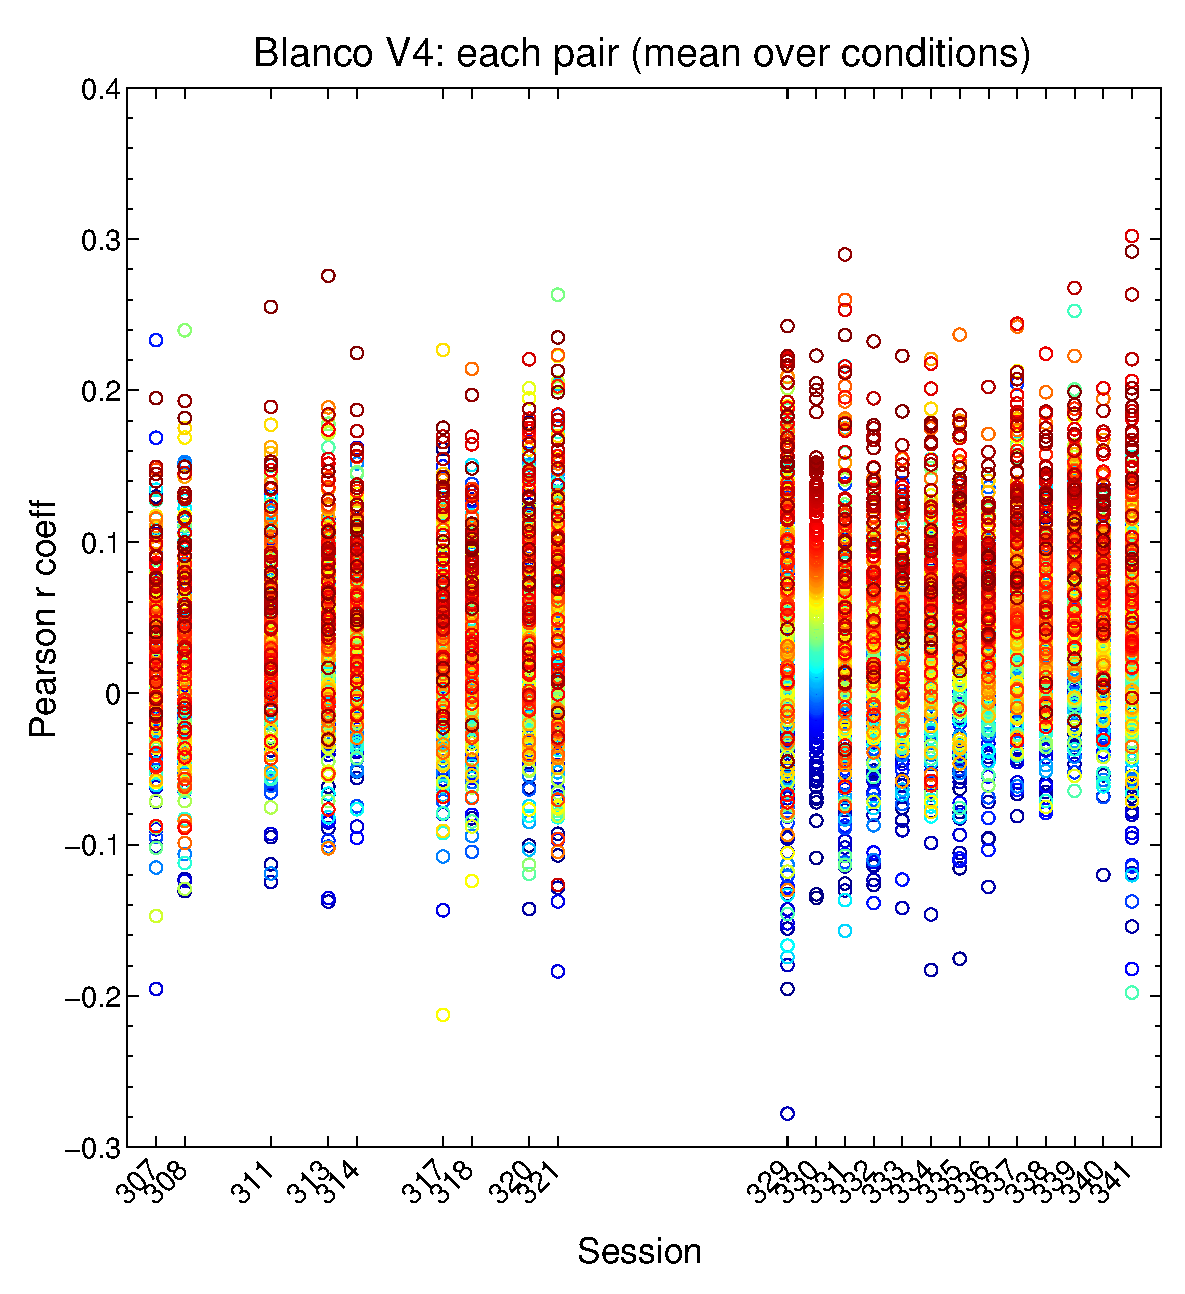
\includegraphics[width=\linewidth]{%
% % ./figs/decoding/rcoef_sess_pairsmeanc_v4_blanco.eps}
% %     \end{subfigure}
% %     ~~
% %     \begin{subfigure}[b]{0.5\linewidth}
% %         \centering
% %         \caption{}
% %         \label{fig:noise_r_j4_pmc}
% %         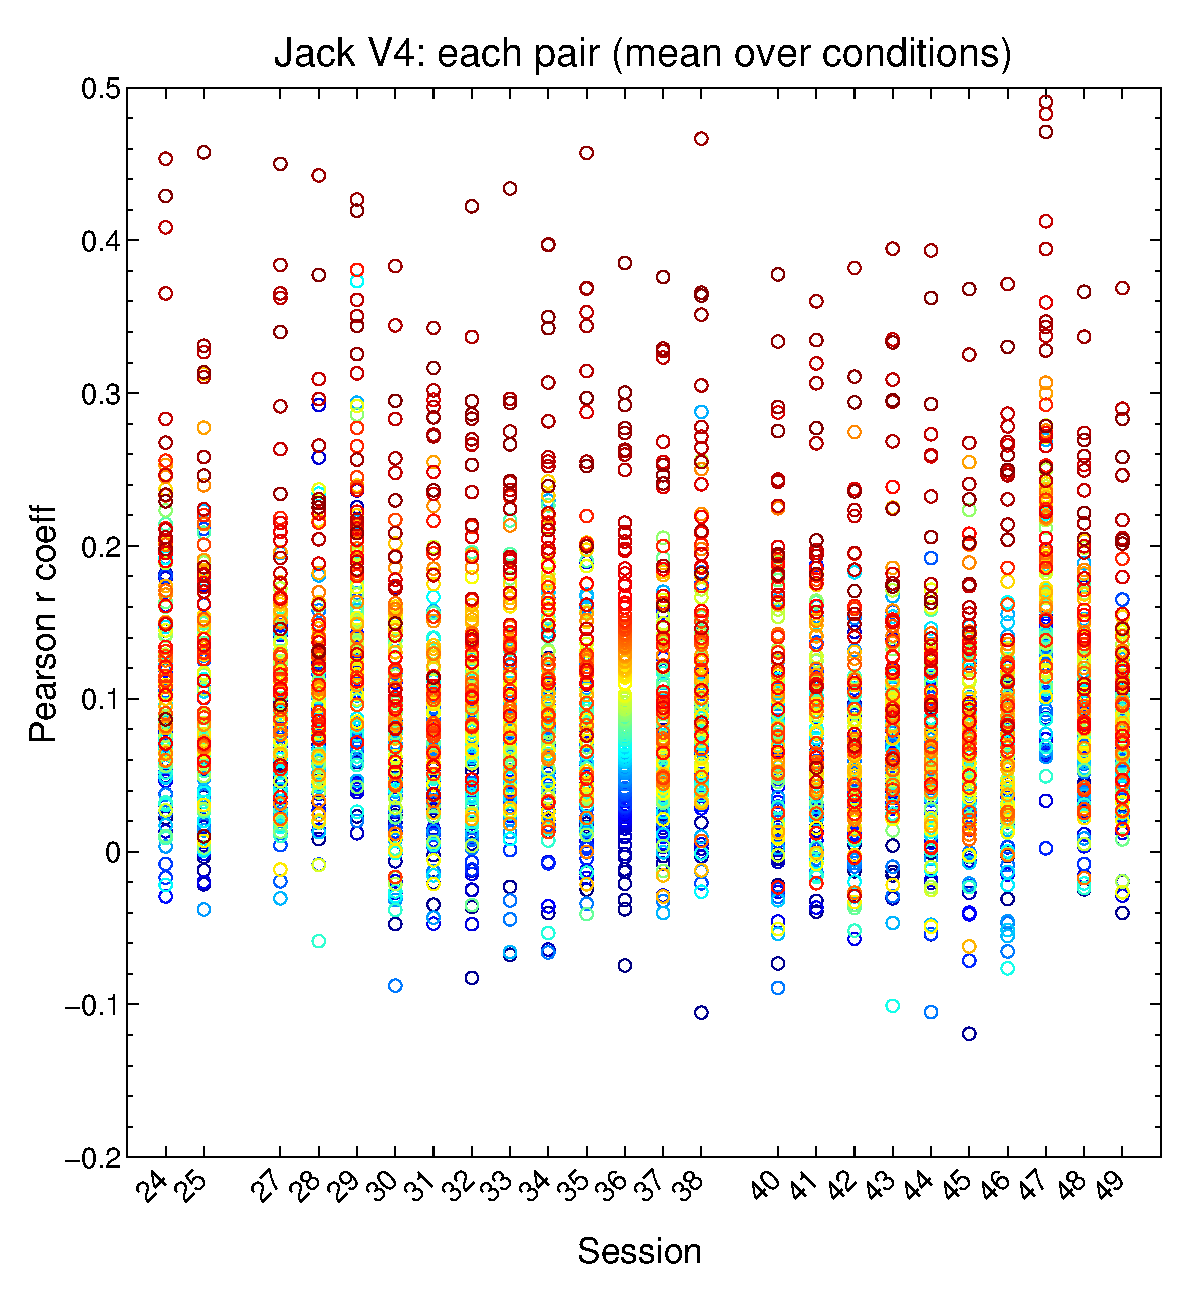
\includegraphics[width=\linewidth]{%
% % ./figs/decoding/rcoef_sess_pairsmeanc_v4_jack.eps}
% %     \end{subfigure}
% %     \caption{Noise correlations for each pair, meaned across the 14 conditions.
% % \protect\subref{fig:noise_r_b1_pmc}: Blanco V1.
% % \protect\subref{fig:noise_r_j1_pmc}: Jack V1.
% % \protect\subref{fig:noise_r_b4_pmc}: Blanco V4.
% % \protect\subref{fig:noise_r_j4_pmc}: Jack V4.
% % Colour is assigned by sorting the pairs into ascending order for one of the sessions near the middle of the training period.
% % The degree of session-to-session correlation of the noise correlation can hence be inferred by visual inspection.
% % }
% %     \label{fig:noise_r_pmc}
% % \end{figure}


% ----------------------------------------------
\clearpage
\section{Discussion}
% ----------------------------------------------

Based on data from Jack V4, one might conclude our results to offer some coroboration with those of \citet{Gu2011}, since we find a decrease in noise correlations and in increase in decoder performance. However, comparing the perforance of the decoder to a decoder based on shuffled data without the noise correlations present suggests that the improvement in decoder performance is not due to the relatively small reduction in noise correlation observed, but is from other sources.

The data from Jack V1 does not support a ``reduction in noise correlation'' hypothesis either, and indicates that neural spike rates across the V1 population recorded from are no more informative after training than they were before. Together, results from Jack V1 and V4 suggest that information in V1 is consistent throughout training, but the ability of V4 to read out the information in V1 improves over the same period, leading to an improvement in behavioural performance.

However, these findings are not supported by the data from Blanco.

% In addition to this, the increase in reponse agreement between our rate-based decoder and the animal's behavioural responses for Jack V4 (Fig.~\ref{fig:dec_j4_alla}) indicates the monkey is increasingly relying on the activity from the channels which were recorded from in V4 in order to make its decisions about the presented stimulus contrast.

For both animals, from the data from V4 we find there is a statistically significant level of agreement between decoded and behavioural trial-to-trial responses after training but not before, which shows the neural activity in V4 and the behavioural resposes are correlated. This implies that the monkey becomes dependent on the activity of the population of neurons for which the recordings are representative. That the agreement is better without shuffling could be taken to mean the neural correlations are important in the determination of the animal's response, however shuffling does by its very nature destroy the correspondence between the trials given to the decoder and those experienced by the animal.
